% Ltex language=en
% \documentclass[12pt, 1p, review, number]{elsarticle}
\documentclass[3p,twocolumn,preprint]{elsarticle}
%\documentclass[10pt,a4paper,3p,twocolumn]{elsarticle}
% \documentclass[5p,preprint,twocolumn]{elsarticle}
%----------------------------------------------------------------------
%                     Loading of packages
%----------------------------------------------------------------------

% for cutting words
\usepackage[utf8]{inputenc}
% a font close to that chosen by Elsevier
\usepackage[bitstream-charter]{mathdesign}
\usepackage{mathtools, cuted}
% for accentuated characters
%\usepackage[T1]{fontenc}
\geometry{top=2cm,left=1.5cm,bottom=2cm,right=1.5cm}
\usepackage{multicol}
% For treating ps:
\usepackage{psfrag}
% For subfigures
\usepackage{subcaption}
\usepackage{placeins}
% For tables
\usepackage{array}
\usepackage{multirow}
\usepackage{hhline}
\usepackage{colortbl}
\usepackage{tabulary}
\usepackage{etoolbox}
% For citations
\usepackage[numbers]{natbib}
%\biboptions{longnamesfirst,angle,semicolon}
%\citetstyle{nature}
% For color
\usepackage{color}
\usepackage{xcolor}
% For spacing
\usepackage{setspace}
%\doublespacing
\singlespacing
%\onehalfspacing
% For maths
\usepackage{amsmath, amsfonts}
\usepackage[squaren,ashgrey]{SIunits}
% For Line numbering
\usepackage[pagewise,modulo]{lineno}
%\linenumbers
% For special characters
\usepackage{pifont}
%
\usepackage[pagebackref,colorlinks=True]{hyperref}
\usepackage{wasysym}
\usepackage{color}
\usepackage{cleveref}
\crefformat{figure}{(Fig.~#2#1#3)}
\usepackage{hyperref}
\usepackage[hyperpageref]{backref}
\usepackage{lipsum}
\usepackage{booktabs} % To thicken table lines
% \usepackage{widetext}
\usepackage{float}
\usepackage{empheq}
\usepackage{textcomp}
\usepackage{multicol}
\usepackage{graphicx}

%----------------------------------------------------------------------
%                     Commands
%----------------------------------------------------------------------
\renewcommand*{\overrightarrow}[1]{\vbox{\halign{##\cr \tiny\rightarrowfill\cr\noalign{\nointerlineskip\vskip1pt}$#1\mskip2mu$\cr}}}
%% Degree character
\DeclareTextSymbol{\degr}{T1}{6}
\newcommand{\degre}[0]{\degr C}
\DeclareUnicodeCharacter{2212}{-}
% MPam^0.5 character
\newcommand{\mpa}[0]{\mbox{MPa}\sqrt{\mbox{m}}}
%mettre de nouilles sous les tenseurs
\newcommand{\ve}[1]{{\underline{#1}}}
\def\ten#1{\oalign{$#1$\crcr\hidewidth$\scriptscriptstyle\sim$\hidewidth}} 
% derivee seconde
\newcommand{\fda}[2]{\displaystyle \frac{\partial\,{#1}}{\partial\, {#2}}}
% et al. for citations
\newcommand{\etal}[0]{{\em et al.}}
\renewcommand*\contentsname{\large{Table of contents}}
\def \hfillx {\hspace*{ -\linewidth} \hfill} % remplir espacement horizontal entre deux sous-figures de façon à remplir toute la largeur du texte.
% \renewcommand{\degree}[1]{${#1}^\circ$} % °

%----------------------------------------------------------------------
%                     Colors
%----------------------------------------------------------------------
\definecolor{ashgrey}{rgb}{0.7, 0.75, 0.71}
%----------------------------------------------------------------------
%                     Pre-Document
%----------------------------------------------------------------------
\journal{Applied Energy}
%----------------------------------------------------------------------
%                     Document
%----------------------------------------------------------------------
\begin{document}

\tableofcontents

\begin{frontmatter}

%% Title, authors and addresses

%% use the tnoteref command within \title for footnotes;
%% use the tnotetext command for theassociated footnote;
%% use the fnref command within \author or \address for footnotes;
%% use the fntext command for theassociated footnote;
%% use the corref command within \author for corresponding author footnotes;
%% use the cortext command for theassociated footnote;
%% use the ead command for the email address,
%% and the form \ead[url] for the home page:
%% \title{Title\tnoteref{label1}}
%% \tnotetext[label1]{}
%% \author{Name\corref{cor1}\fnref{label2}}
%% \ead{email address}
%% \ead[url]{home page}
%% \fntext[label2]{}
%% \cortext[cor1]{}
%% \address{Address\fnref{label3}}
%% \fntext[label3]{}

\title{Ear canal dynamic motion piezoelectric energy harvester using a bistable resonator cycled by coupled hydraulic switches made of collapsed flexible tubes.}

%% use optional labels to link authors explicitly to addresses:
%% \author[label1,label2]{}
%% \address[label1]{}
%% \address[label2]{}


\address[symme]{Laboratoire SYMME - Université Savoie Mont Blanc, 7 Chemin de Bellevue, 74940, Annecy}
\address[critias]{Université du Québec - École de technologie supérieure, 1100 Rue Notre-Dame Ouest, Montréal, QC, H3C 1K3}


\author[symme]{Tigran AVETISSIAN}
\author[symme]{Fabien FORMOSA}
\author[symme]{Adrien BADEL}

\author[critias]{Michel DEMUYNCK}
\author[critias]{Aidin DELNAVAZ}
\author[critias]{Jérémie VOIX}


\begin{abstract}
%% Text of abstract
\end{abstract}

\begin{keyword}
%% Keywords
\end{keyword}

\end{frontmatter}

%\linenumbers

%% main text
 % Ltex language=en
\begin{table*}
\begin{large}
	\begin{center}
		Nomenclature	\\
		\noindent\makebox[\linewidth]{\rule{\textwidth}{0.4pt}}
	\end{center}
\end{large}		
% \end{table*}
\begin{minipage}{.5\textwidth}
%%%%%%%%%%%%%%%%%%%%%%%%%%%%%%%%%%%%%%%
% \begin{table}[!h]
	\begin{tabular}{ c  m{6cm} }
		\textbf{Subscripts}      &                                                         \\
		APG                      & Amplified piezoelectric generator                       \\
		BB                       & Buckled beam                                           \\
		BR                       & Bistable resonator                                      \\
		GB                       & Guide beam                                             \\
		HA                       & Hydraulic amplifier                                     \\
		HC                       & Hydraulic cylinder                                      \\
		HV                       & Hydraulic valve                                         \\
		PFF						 & piezoelectric force factor  \\
		\textbf{Roman letters}   &                                                         \\
		$a$ [m]                  & HV bending lever arm                                    \\
		$a_h$ [-]                & Hydraulic amplification level                           \\
		$Cf$ [Pa.s$^2$.m$^{-6}$]         & Pressure loss coefficient                               \\
		$Cf_0$ [Pa.s$^2$.m$^{-6}$]       & Opened HV pressure loss coefficient                     \\
		$Cf_c$ [Pa.s$^2$.m$^{-6}$]       & Closed HV pressure loss coefficient                     \\
		$C_p$ [F]                & APG internal capacity                                   \\
		$D_h$ [m]                & Hydraulic diameter of the HV                            \\
		$D_{hc}$ [m]             & Hydraulic cylinder internal diameter                    \\
		$D_r$ [m]                & HV rigid sheath diameter                                \\
		$E_d$ [J]                & Global dissipated energy                                \\
		$E_e$ [J]                & Harvested electric energy                               \\
		$E_{hyd}$ [J]            & Available hydraulic energy from earplug                 \\
		$F_{br}$ [N]             & BR counter reaction force                               \\
		$f_0$ [Hz]				 &	BR natural resonance frequency						   \\
		$K$ [N/m]                & APG stiffness                                           \\
		$K_{bb}$ [N/m]           & 8 BB's stiffness                                        \\
		$K_{eq}$ [N/m]           & Equivalent stiffness seen from the APG                  \\
		$K_{gb}$ [N/m]           & GB stiffness                                            \\
		$K_{HV}$ [N.m/rad]        & HV stiffness                                            \\
		$K_s$ [N/m]              & Spring stiffness                                        \\
		$K_{\varphi}$ [N.m/rad]   & Single hinge stiffness                                  \\
		$k^2$ [-]                & APG electromechanical coupling coefficient              \\
		$k_{sys}^2$ [-]          & Global electromechanical coupling coefficient           \\
		$L$ [m]                  & Distance between 2 BR adjacent hinges                   \\
		$l_0$ [m]                & Distance between 2 BR adjacent hinges on $\vec{x}$ axis \\
	\end{tabular}
% \end{table}
\end{minipage}
\begin{minipage}{.5\textwidth}
% \begin{table}[!h]
\begin{tabular}{ c  m{6cm} }
		$m$ [kg]			     & BR dynamic mass 										   \\
		$p_c$ [Pa]               & comfort pressure                                        \\
		$p_{hc}$ [Pa]            & Hydraulic cylinder internal pressure                    \\
		$S_{hc}$ [Pa]            & Hydraulic cylinder internal section                     \\
		$q$ [m$^3$/s]            & Flow rate                                               \\
		$R_l$ [$\Omega$]         & Load resistance                                         \\
		$P_e$ [W]                & Harvested electric power                                \\
		$Q$ [-]                  & BR quality factor                                       \\
		$r_{Cf}$ [-]             & Hydraulic restriction coefficient                       \\
		$x_m$ [m]                & BR mass position                                        \\
		$x_{hc}$ [m]             & HC piston position                                      \\
		$x_m$ [m]                & BR mass position                                        \\
		$x_0$ [m]                & BR buckling height                                       \\
		$U_p$ [V]                & APG tension                                             \\
		\textbf{Greek letters}   &                                                         \\
		$\alpha$ [N/V]           & piezoelectric force coefficient                         \\
		$\Delta p_{ear}$ [Pa]    & Earplug pressure variation                              \\
		$\Delta V_{ear}$ [m$^3$] & Earplug volume variation                                \\
		$\epsilon$ [-]           & BR buckling level                                       \\
		$\eta_{br}$ [-]          & BR energy conversion efficiency                         \\
		$\eta_g$ [-]             & Harvester energy conversion efficiency                  \\
		$\theta$ [rad]           & HV bending angle                                        \\
		$\mu$ [N.s/m]             & Air dynamic viscosity                                   \\
		$\mu_{hc}$ [N.s/m]        & HC viscous loss coefficient                             \\
		$f_d$ [N.s/m]             & Dry friction loss coefficient                           \\
		$\varphi$ [rad]			 & BR hinge rotational angle							   \\
		$\omega_0$ [rad/s]       & BR natural angular frequency                            \\
		\textbf{Indexes}         &                                                         \\
		$\square_a$              & Active hydraulic branch                                 \\
		$\square_b$              & \emph{Bottom} side hydraulic branch ($x <0$)            \\
		$\square_c$              & Closed HV state              						   \\
		$\square_i$              & \emph{Top} side hydraulic branch ($x >0$)               \\
		$\square_o$              & Opened HV state             							   \\
		$\square_t$              & Inactive hydraulic branch                               \\
		$\square_{max}$          & Upper value                                             \\
		$\square_{min}$          & Lowest value                                            \\
	\end{tabular}
% \end{table}
\end{minipage}
%%%%%%%%%%%%%%%%%%%%%%%%%%%%%%%%%%%%%%%
% \begin{table*}
		\begin{center}
			\noindent\makebox[\linewidth]{\rule{\textwidth}{0.4pt}}
		\end{center}
\end{table*}
%/!\/!\/!\/!\/!\/!\/!\/!\/!\/!\/!\/!\/!\/!\/!\/!\/!\/!\/!\/!\/!\/!\/!\/!\%
\section{INTRODUCTION}
\label{INTRODUCTION}
%/!\/!\/!\/!\/!\/!\/!\/!\/!\/!\/!\/!\/!\/!\/!\/!\/!\/!\/!\/!\/!\/!\/!\/!\%
The growing use of wireless devices and the miniaturization of electronic circuits have led to significant progress on the energy consumption of mobile devices on the human body environment. Energy harvesting methods have been studied in order to complement their power supply and enhance the autonomy of the batteries. In-ear devices such as hearing aids and cochlear implants are powered by disposable cells or rechargeable batteries. The energy consumption of the best integrated devices in the literature rises up to $17$J for a 10 hours daily use \cite{Scherer2019,Yip2015,Kulah2022}. Woodruff \emph{et al.} underlined that patients using hearing aids sometimes struggle to change and select batteries for their devices \cite{Woodruff2021}. Another statistical study revealed that the majority of hearing aids and cochlear implants users prefer disposable batteries for the long autonomy, but would have liked rechargeable solutions if the battery cycle was sufficient to complete the day \cite{PracticesAudiology2016}. Also, the long term use makes the rechargeable solutions a more economical and more ecological choice compared to the disposable cells. These arguments motivated the development of energy harvesting systems.

The common energy sources are solar or wind energy but their availability in the low size environment of the application context makes them not suitable for exploitation. The activities of the human body generate a considerable amount of energy of different natures. Among them, the electrochemical energy from the inner ear \cite{Mercier2012}, the kinetic energy from walking or head movements \cite{Azimi2021,Smilek2016}, the body heat thermal energy \cite{Kim2014}, the strain energy from the skin deformation \cite{Jin2021} could be harvested for in-ear applications. An interesting energy source for cochlear implants or hearing aids appears to be the ear canal mechanical deformation as it is directly located in the area of the application. Delnavaz \emph{et al.} first showed in 2012 that the jaw movements changes de ear canal geometry during mastication. Carioli \emph{et al.} then used a customized earplug molding technic with a 3D scanner to reveal a global bending movement and a local compression area in the ear canal during mastication \cite{Carioli2016}. These two mechanical deformations represent a potential energy source that can be exploited.

Delnavaz \emph{et al.} developed a flexible piezoelectric harvester made of a silicon earplug with a PVDF layer \cite{Delnavaz2013}. The earplug has been molded on the subject in order to maximize the contact surface with the ear canal. The harvester is capable of exploiting both the flexion and the compression energy sources. The experimental prototype was able to extract $44$µJ from a mastication cycle. The soft materials facilitate the bio-integration of the harvester but the PVDF low electromechanical coupling coefficient could have led to poor energy conversion efficiency. A hydro-electromagnetic energy harvester was also developed by the same researchers \cite{Delnavaz2012}. The energy is extracted by a liquid filled earplug whose internal volume vary as a result of the radial compression of the ear canal internal walls during the jaw movements. This variation put into motion a moving magnet translating in a water column surrounded by a coil. The generated energy experimentally amounts to 0.2µJ per mastication cycle. The prototype appeared to be less efficient than the PVDF earplug. This could be explained by the poor power generation of the electromagnetic transduction for a low frequency energy source (1.57Hz) and a small scale application \cite{Kulah2008,Priya2017}. However, the hydraulic transmission allows the use of more complex and voluminous technological solutions since the energy becomes available outside the small ear canal volume.

Based on the analysis of the literature, we propose a new solution optimizing the energy conversion efficiency to maximize the harvested energy from the ear canal dynamic motion. The next section states on the hydraulic energy source characterization and on the harvesting strategy that we adopted. Section \ref{sec:HARVESTER PRESENTATION AND OPERATION PRINCIPLE} presents the harvester and describes its operation principle. Section \ref{sec:SYSTEM MODELING} details the global system modeling and section \ref{sec:NUMERICAL MODEL AND SIMULATIONS} presents the numerical simulation of the theoretical behavior of the harvester. Then section \ref{sec:EXPERIMENTAL CHARACTERIZATIONS OF THE ELECTROMECHANICAL CONVERTER} then exposes the experimental validation performed on the electromechanical converter stage and section \ref{sec:EXPERIMENTAL APPROACH FOR THE HV DESIGN} shows the experimental approach for the design of the hydraulic valves for the system cycling. Then, section \ref{sec:MODEL RECALIBRATION WITH EXPERIMENTAL DATA} presents the experimentally adjusted global harvester model and discusses this work major contributions and the harvester potential. Finally, a conclusion is stated.

%/!\/!\/!\/!\/!\/!\/!\/!\/!\/!\/!\/!\/!\/!\/!\/!\/!\/!\/!\/!\/!\/!\/!\/!\%
\section{ENERGY SOURCE AND HARVESTING STRATEGY}
\label{sec:THE ENERGY SOURCE AND HARVESTING STRATEGY}
%/!\/!\/!\/!\/!\/!\/!\/!\/!\/!\/!\/!\/!\/!\/!\/!\/!\/!\/!\/!\/!\/!\/!\/!\%
    %///////////////////////////////////////////// 
	\subsection{The energy source}	
	\label{The energy source}
    %/////////////////////////////////////////////
Human tissue requires soft flexible materials in order to extract the ear canal deflection energy without causing discomfort. However, flexible transducers admit low energy conversion efficiency as a part of the extracted energy is dissipated in the elastic non-active material. Additionally, the low frequency of mastication makes it difficult to use resonant structures that generally admit better conversion efficiencies than low frequency solutions \cite{Ashraf2011}. Thus, the traditional transducing methods are not suitable enough for the application.

To date, the best solution proposed in the literature consists on using soft materials as the piezoelectric PVDF earplug previously introduced \cite{Delnavaz2013}. The low mechanical impedance of the soft tissue in fact limits the use of more effective rigid piezoelectric materials.

The hydraulic extraction strategy proposed in \cite{Delnavaz2012} is less effective than the piezoelectric earplug but allows to transmit the energy outside the ear canal and benefit so from larger effective space. The latter is in fact essential as it becomes then possible to implement an impedance adaption stage and more effective transducing methods that could not fit directly inside the ear canal restricted volume. In fact, Marin \emph{et al.} demonstrated that the power generated by piezoelectric or electromagnetic transducers is as much better as the effective volume of transducing material is high \cite{Marin2011}. The present work is then based on the exploitation of the ear canal by a liquid filled earplug. As energy source, it can be assimilated to a micro pump characterized by its volume variation $V_{ear}$ and pressure variation $p_{ear}$. In order to optimize the energy extraction, the earplug must fit the ear canal wall. Turcot \emph{et al.} demonstrated that the initial pressurization must reach a minimum of $14$kPa to achieve a good fit \cite{TURCOT2011}. Bouchard-Roy \emph{et al.} studied the dynamic pressure variation inside the earplug for different initial pressurization levels \cite{Bouchard-Roy2020}. A maximum of $\text{max}(\Delta p_{ear})=12$kPa of dynamic pressure variation, with a $28$kPa of initial pressurization, has been noted during the mastication for seven subjects. Besides, the temporal evolution of the volume variation $\Delta V_{ear}$ has been estimated in \cite{Delnavaz2012} and the result for a mastication cycle is presented on figure \ref{fig:deltaV_ear}.
%%%%%%%%%%%%%%%%%%%%%%%%%%%%%%%%%%%%%%
\begin{figure}[!htbp]
	\centering
	\captionsetup{justification=centering}
	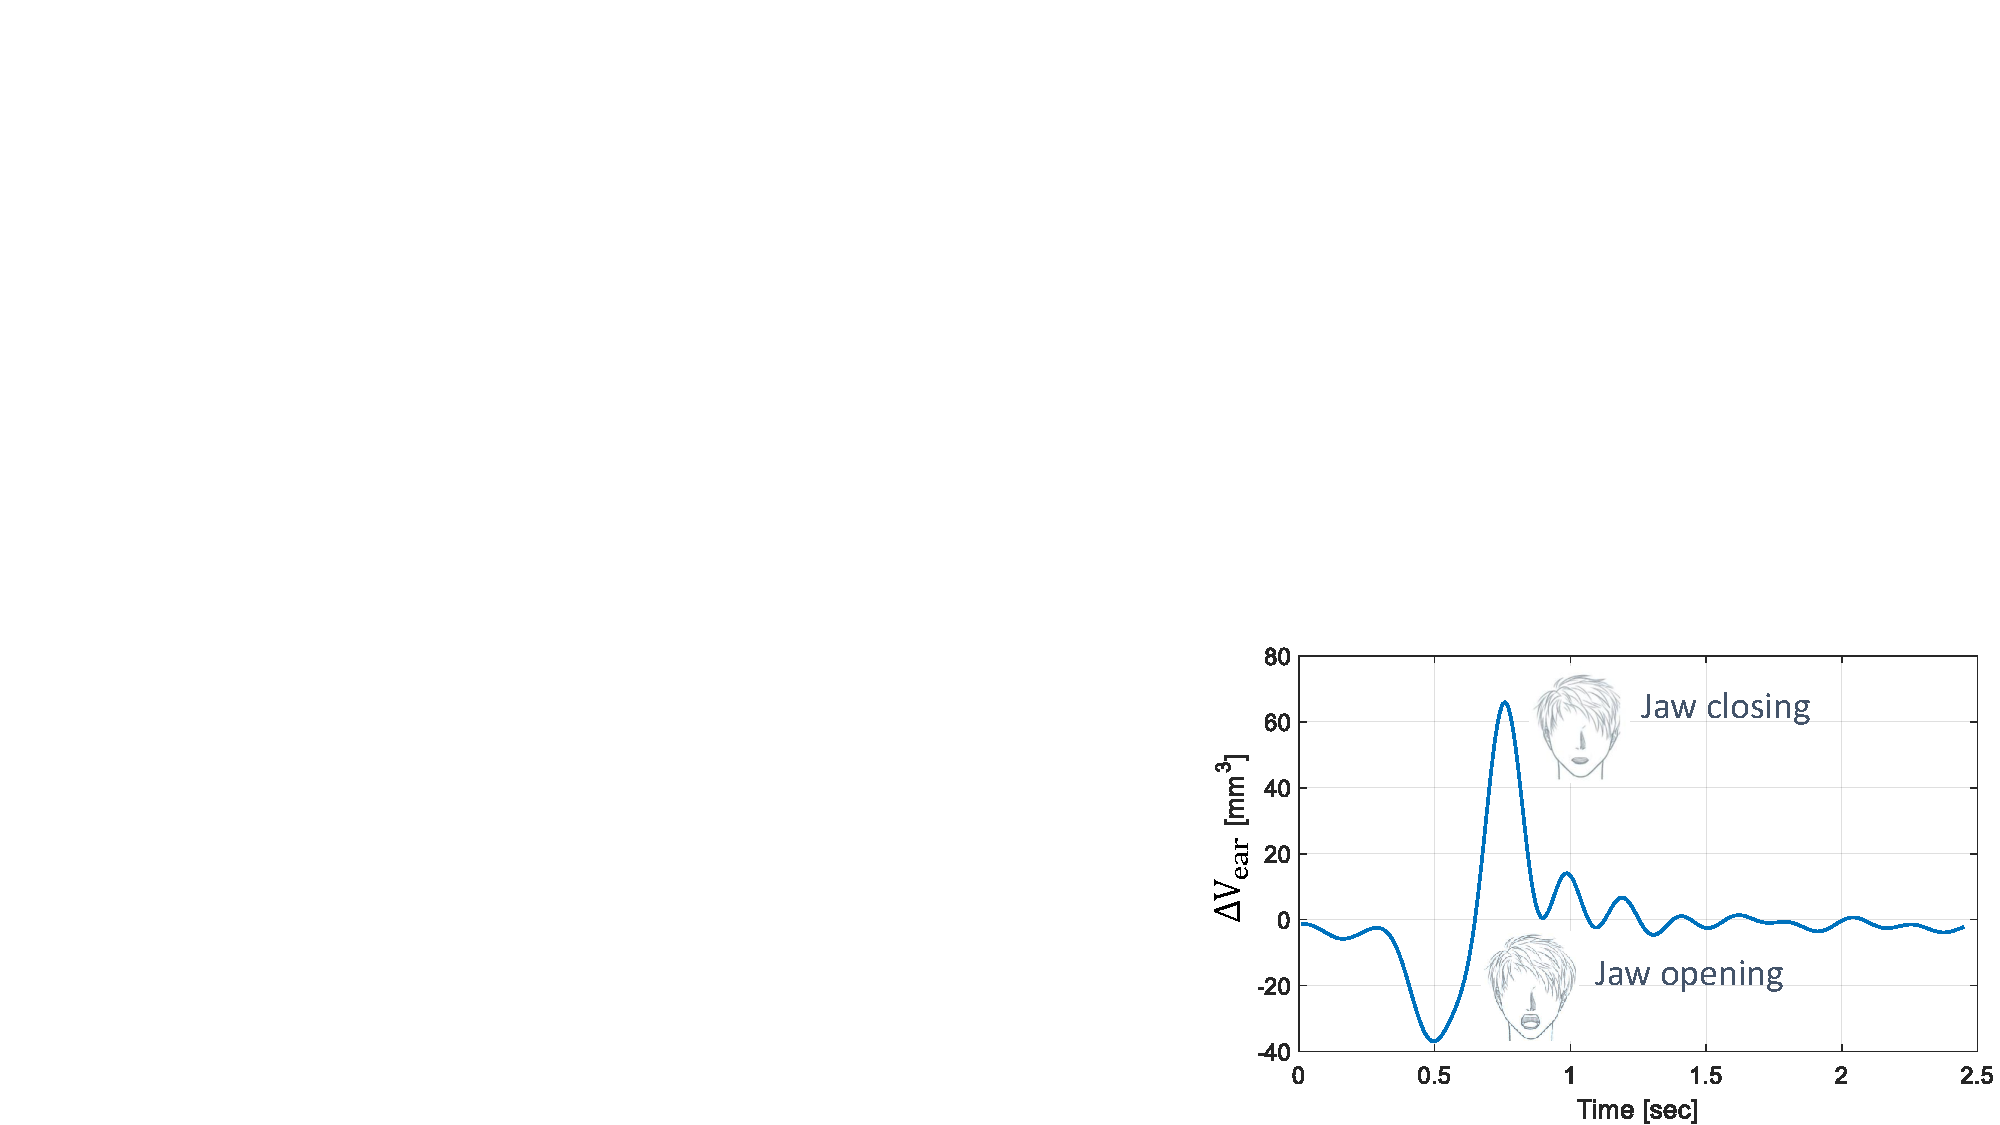
\includegraphics[trim={20.5cm 0cm 0cm 10.8cm},clip, width=0.4\textwidth]{figures/deltaV_ear.pdf}
	\caption{Ear canal volume variation for one mastication cycle}
	\label{fig:deltaV_ear}
\end{figure}
%%%%%%%%%%%%%%%%%%%%%%%%%%%%%%%%%%%%%%

The earplug operation characteristic behavior has not been studied yet. Thus, the evolution of the volume variation $\Delta V_{ear}$ is not well known as a function of the pressure variation $\Delta p_{ear}$. Then, considering the pressure and volume variation levels from \cite{Delnavaz2012} and \cite{Bouchard-Roy2020}, the equation \ref{eq:max_hydraulic_energy} approximates an upper limit for the extractable hydraulic energy with the maximum values of $\Delta p_{ear}$ et $\Delta V_{ear}$ that have been recorded, i.e. $p_c=12kPa$ and $(\Delta V_{ear})_{max}=60$mm$^3$. $p_c$ stands for the comfort pressure by assuming that the user could feel discomfort if $\Delta p_{ear}>p_c$. The energy estimation presumes that the earplug is a perfect flow rate source, which is a theoretical hypothesis leading to $0.9$mJ available from one mastication. Based on 2200 mastication cycles per day, according to \cite{Goll2011}, there would be $2$mJ available per day, per ear. This amount of energy could theoretically enhance supply $23.5$\% of the $17$J of needed for the state of the art of cochlear implants \cite{Kulah2022}. Further research in both domains related to hearing aids and energy harvesting could lead to fully autonomous devices in the future.
\begin{align}
	\text{max}(E_{hyd}) = p_c \cdot (\Delta V_{ear})_{max} = 0.9\text{mJ}
	\label{eq:max_hydraulic_energy}
\end{align}

    %///////////////////////////////////////////// 
	\subsection{Harvesting strategy}	
	\label{The harvesting strategy}
    %/////////////////////////////////////////////
Electromagnetic transducers are usually used to harvest energy from kinetic (vibration) energy sources. The power density of electromagnetic transducers decreases as much as the effective volume of transducing material and the frequency of the energy source decrease \cite{Priya2017,Kulah2008}. Also, the fabrication and the integration of the coil and the moving magnet can come out to be difficult as the gap between the two components has to be carefully managed to prevent non-linear unpredicted responses \cite{Caruntu2001}. 

Piezoelectric ceramics appear like good candidates for mechanical energy transduction at small scales, but their high stiffness can limit their use on soft materials as human tissues. Mechanical amplifiers like flextensional structures can nevertheless be used to adapt the stress/displacement levels between the energy source and the transducing stiff material \cite{Abdelnaby2016}. Also, the best energy conversion efficiency for piezoelectric ceramics is achieved for at the transducer resonance. As the mean mastication frequency is estimated to \mbox{$1.57$Hz}, the harvesting system could benefit from a frequency-up conversion stage \cite{Ashraf2011,Peng2021} to increase the frequency of the energy source and so the energy conversion efficiency of the transducer. A majority of the frequency-up systems with piezoelectric transducers use mechanical stops with piezoelectric ceramic cantilevers to reach high frequencies with a good mechanical coupling \cite{Edwards2013,Gu2011,Lee2007}. Stoppers however dissipate energy. Alternative solutions use mechanically bistable resonators (BR) \cite{Vocca2012}. Recent works led to the development and optimization of bistable structures integrating stacked piezoelectric ceramics inside flextensional elastic structures \cite{Huguet2017}. They show enhanced performances due to high electromechanical coupling. The electromechanical converter, composed of a BR with piezoelectric ceramics in a flextensional structure, theoretically offers higher energy conversion efficiency compared to low frequency solutions and/or flexible electromechanical transducers \cite{Abdelnaby2016,Peng2021}.

The hydraulic-mechanic interface can be a hydraulic cylinder (HC). It can store the energy in the frequency-up converter by actuating it at the frequency of human mastication. The amount of extractable energy from the hydraulic source will then depend on the mechanical stage behavior. Before being converted in electricity, the energy is in fact stored in a mechanical potential reservoir. During the low frequency actuation, the forces applied on each side of the HC piston are equal. Equation \ref{eq:hydraulic-mechanic_interface} models the hydraulic-mechanic interface with $x_{m}$ and $ S_{hc}$ being respectively the dynamic mass position on the $\vec{x}$ axis and the HC internal section.
%%%%%%%%%%%%%%%%%%%%%%%%%%%%%%%%%%%%%%
\begin{figure}[!htbp]
	\centering
	\captionsetup{justification=centering}
	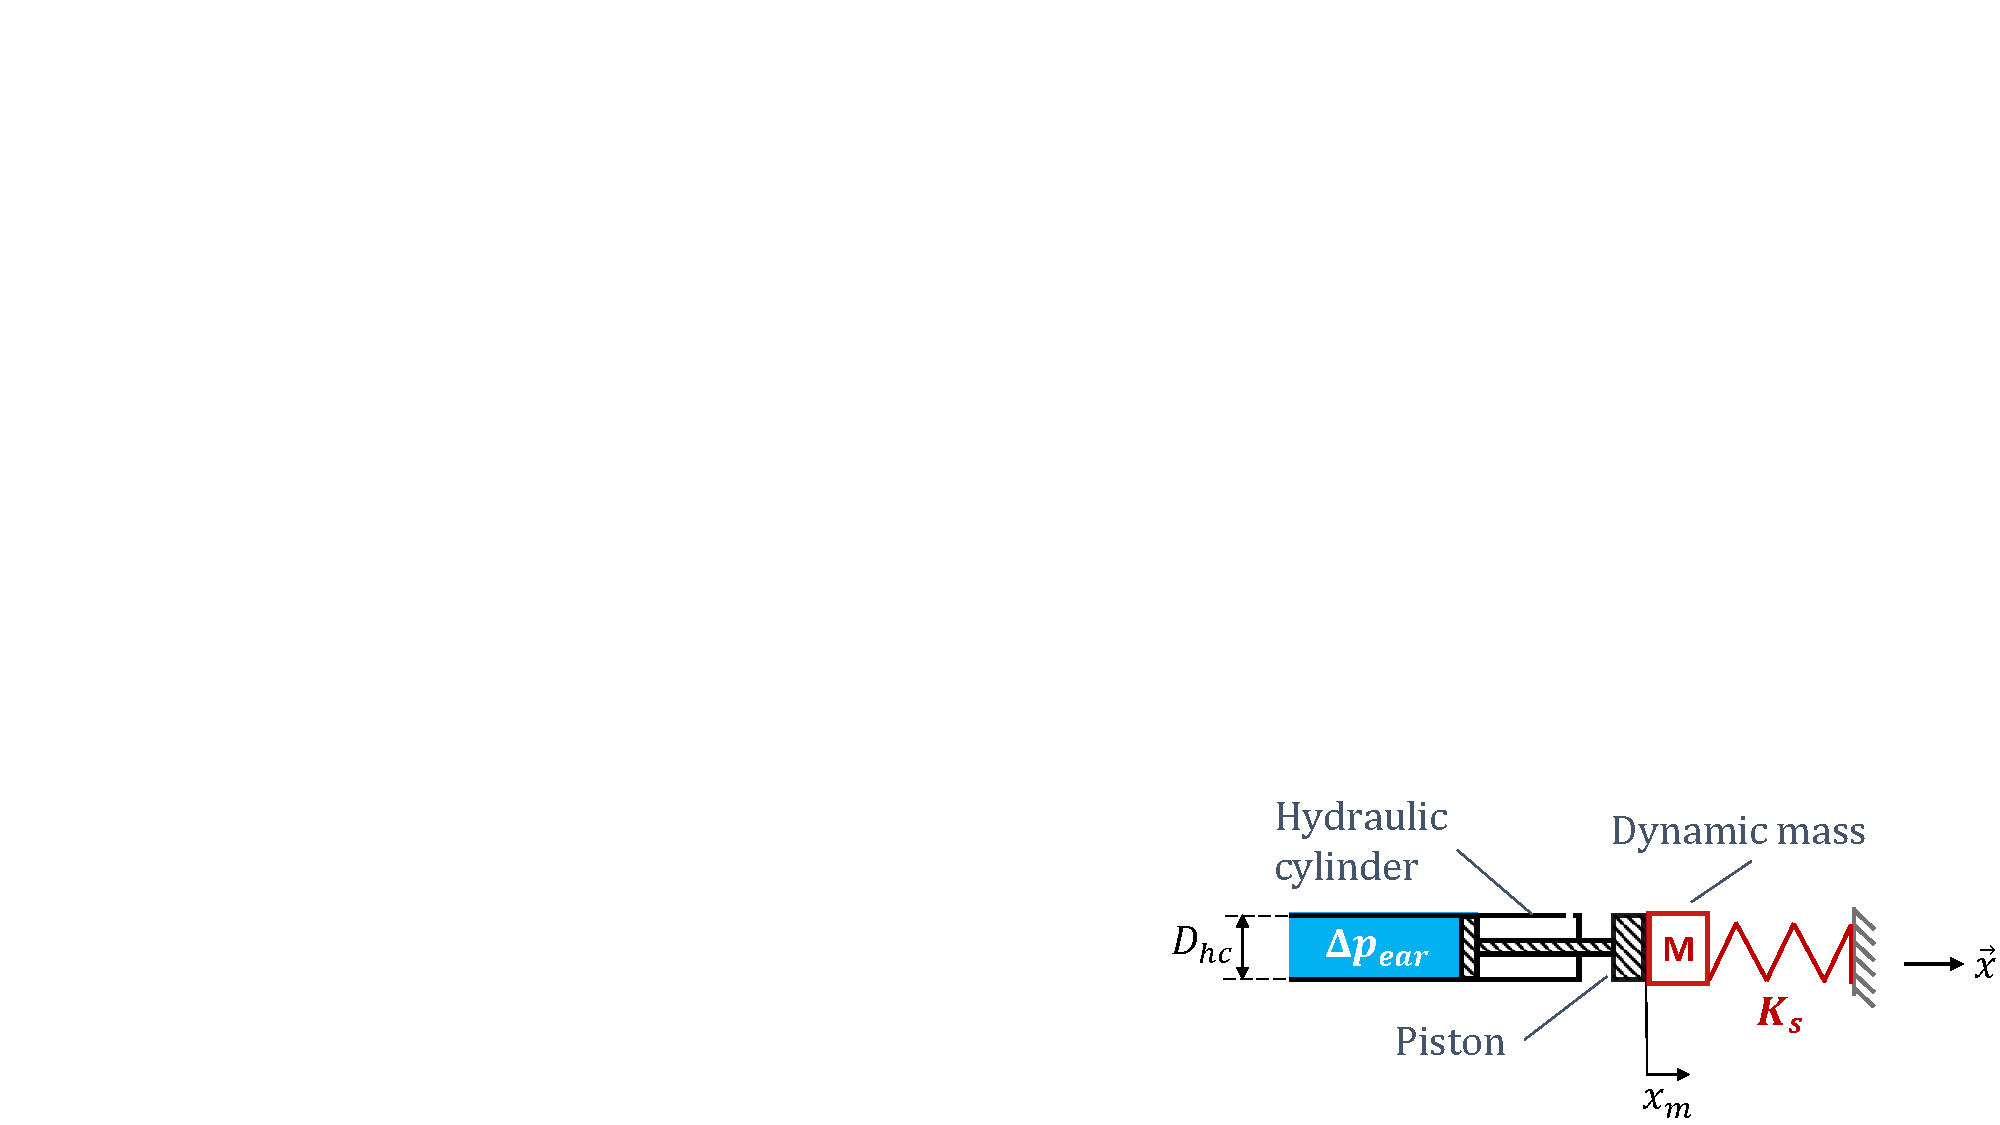
\includegraphics[trim={19.7cm 0cm 0cm 13cm},clip, width=0.7\linewidth]{figures/hydraulic_mechanic_interface.pdf}
	\caption{Hydraulic source exploitation depending on the mechanical load}
	\label{fig:hydraulic_mechanic_interface}
\end{figure}
%%%%%%%%%%%%%%%%%%%%%%%%%%%%%%%%%%%%%%
Therefore, the potential energy stored in a linear resonator from the ideal hydraulic source previously described can be expressed as follows :
\begin{equation}
	Ep_{lin} = \dfrac{K_s\ x_{m}^2}{2} = \dfrac{\Delta p_{ear} \Delta V_{ear}}{2}
	\label{eq:best_linear_soution}
\end{equation}
Thus, the linear solution can theoretically exploit/store a maximum of $50\%$ from the maximum available hydraulic energy ($\text{max}(E_{hyd})$). 

Non-linear elastic potential reservoirs can also be considered. This work presents the energy extraction capability of a BR governed by a Duffing equation. It admits 2 stable equilibrium positions \mbox{$x_m=\pm x_0$}, an unstable one in \mbox{$x_m=0$} and its stiffness depends on its structural buckling level $\epsilon$ defined later in equation \ref{eq:epsilon_def}. The maximum theoretical energy in the BR for a quasi-static actuation is equal to the height of the potential energy barrier $E_{pb}$ when the mass position varies from \mbox{$x_m=\pm x_0$} to \mbox{$x_m=0$} (eq. \ref{eq:Ep_bar}). It will be a fraction $n$ of the upper limit of the available hydraulic energy (eq. \ref{eq:max_hydraulic_energy}) where $n$ has to be maximized. 
\begin{equation}
	E_{pb} = \dfrac{K x_0^2\epsilon^2}{3} = n(p_c \cdot (\Delta V_{ear})_{max})
	\label{eq:Ep_bar}
\end{equation}
We see later that it is inherently capable of exploiting $65$\% from the hydraulic energy source, which is $15$\% better than the best theoretical linear option. Section \ref{sec:SYSTEM MODELING} discusses the details of the modeling and design of the harvester that implements such a non-linear BR as it appeared to be a better solution than the linear approach. 
%/!\/!\/!\/!\/!\/!\/!\/!\/!\/!\/!\/!\/!\/!\/!\/!\/!\/!\/!\/!\/!\/!\/!\/!\%
\section{HARVESTER PRESENTATION AND OPERATION \mbox{PRINCIPLE}}
\label{sec:HARVESTER PRESENTATION AND OPERATION PRINCIPLE}
%/!\/!\/!\/!\/!\/!\/!\/!\/!\/!\/!\/!\/!\/!\/!\/!\/!\/!\/!\/!\/!\/!\/!\/!\%
%%%%%%%%%%%%%%%%%%%%%%%%%%%%%%%%%%%%%%%
\begin{figure*}[!htbp]
	\centering
	\captionsetup{justification=centering}
	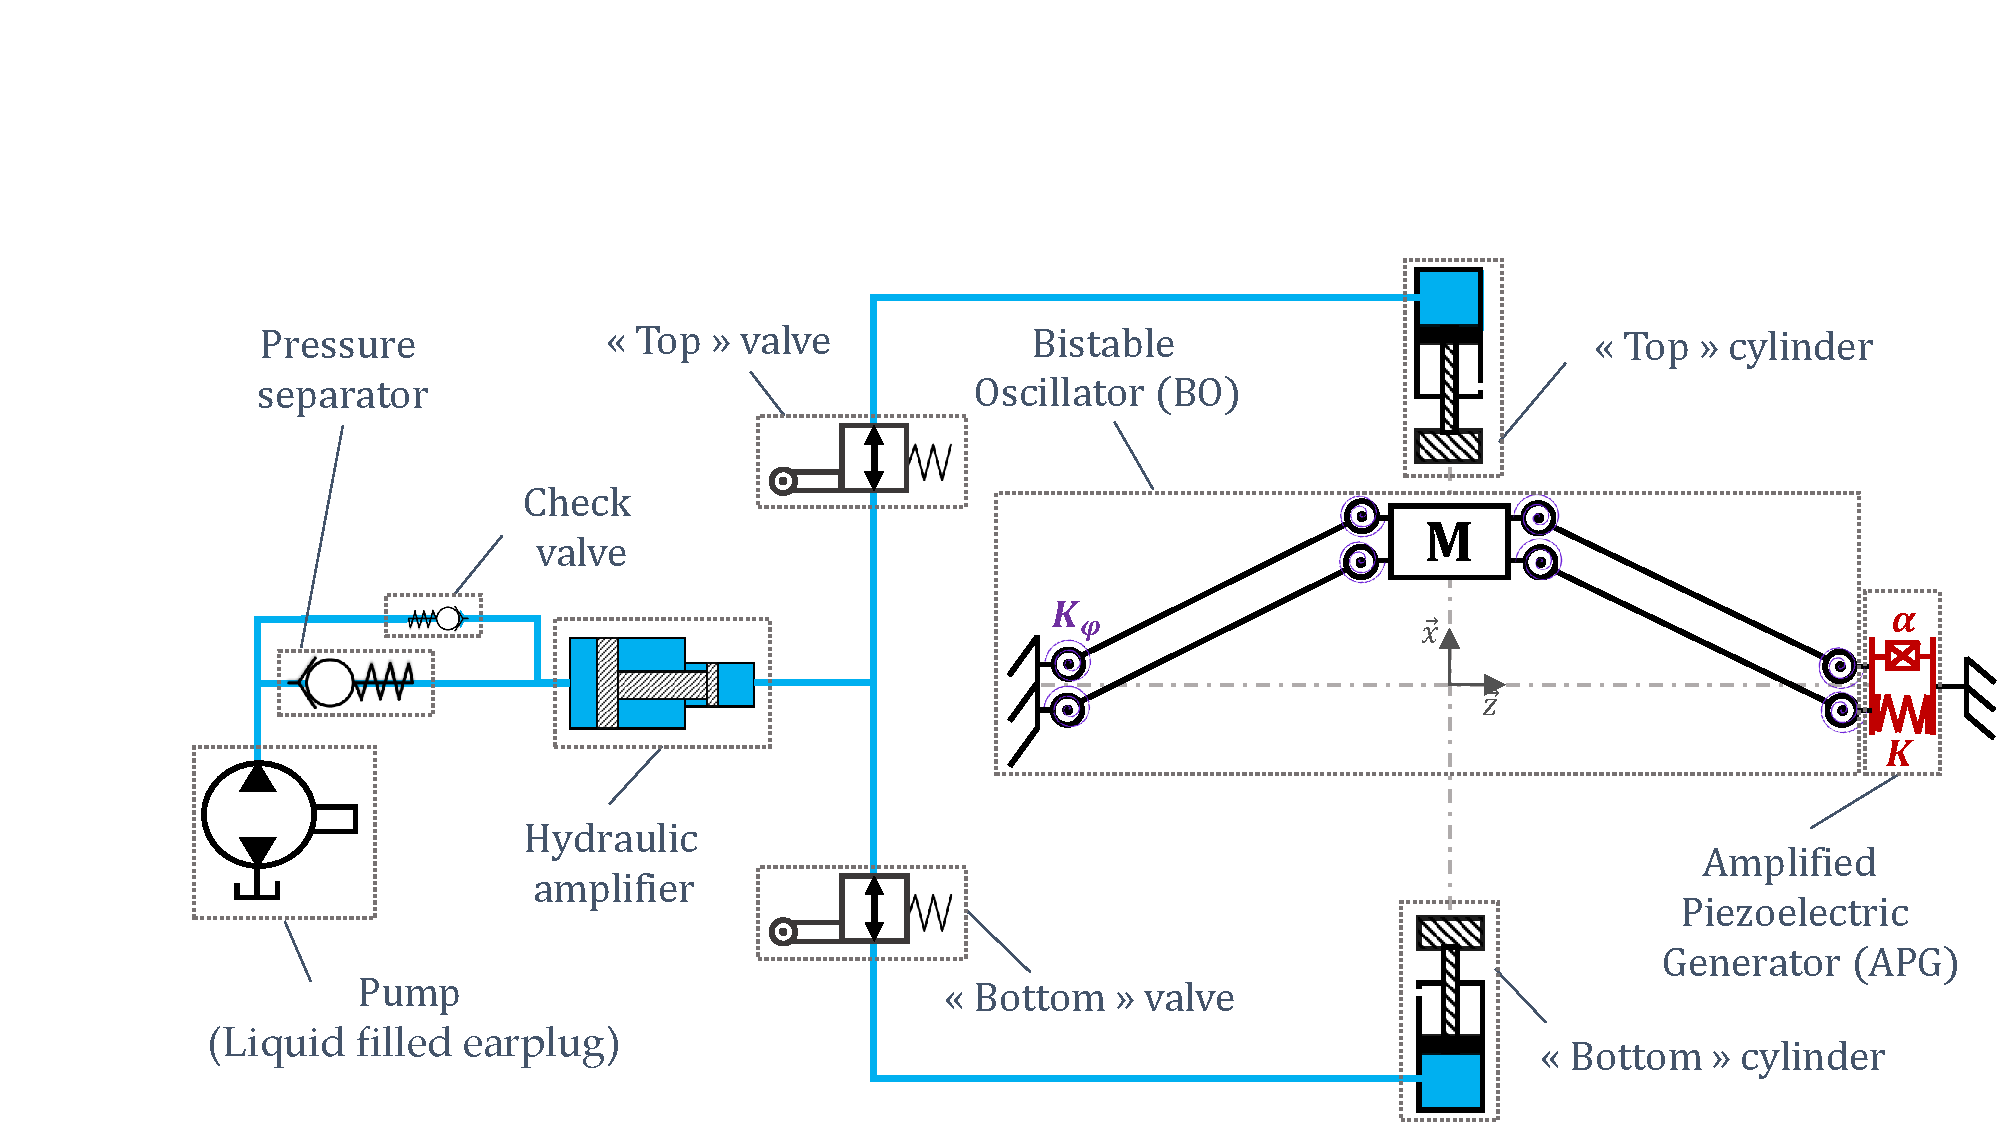
\includegraphics[trim={3.2cm 0cm 0cm 4.3cm},clip, width=0.7\textwidth]{figures/system_presentation.pdf}
	\caption{Schematic presentation of the frequency-up piezoelectric harvester exploiting the ear canal geometry variation} 
	\label{fig:system_presentation}
\end{figure*}
%%%%%%%%%%%%%%%%%%%%%%%%%%%%%%%%%%%%%%%
The figure \ref{fig:system_presentation} presents a schematic view of the energy harvesting system. It uses a liquid filled earplug to transmit the energy outside the ear canal. To maximize the efficiency, the system integrates a frequency-up conversion stage obtained by a BR. The latter is associated with an amplified piezoelectric generator (APG) \cite{CEDRATTECHNOLOGIES2022} made of a flextensional elastic APX4 steel \cite{AUBERT&DUVAL2022} structure containing stacked lead zirconate titanate (PZT) ceramics (fig. \ref{fig:APG}).
%%%%%%%%%%%%%%%%%%%%%%%%%%%%%%%%%%%%	
\begin{figure}[!htb]
	\begin{center}
		\begin{subfigure}[t]{0.5\linewidth}
			\captionsetup{justification=centering}
			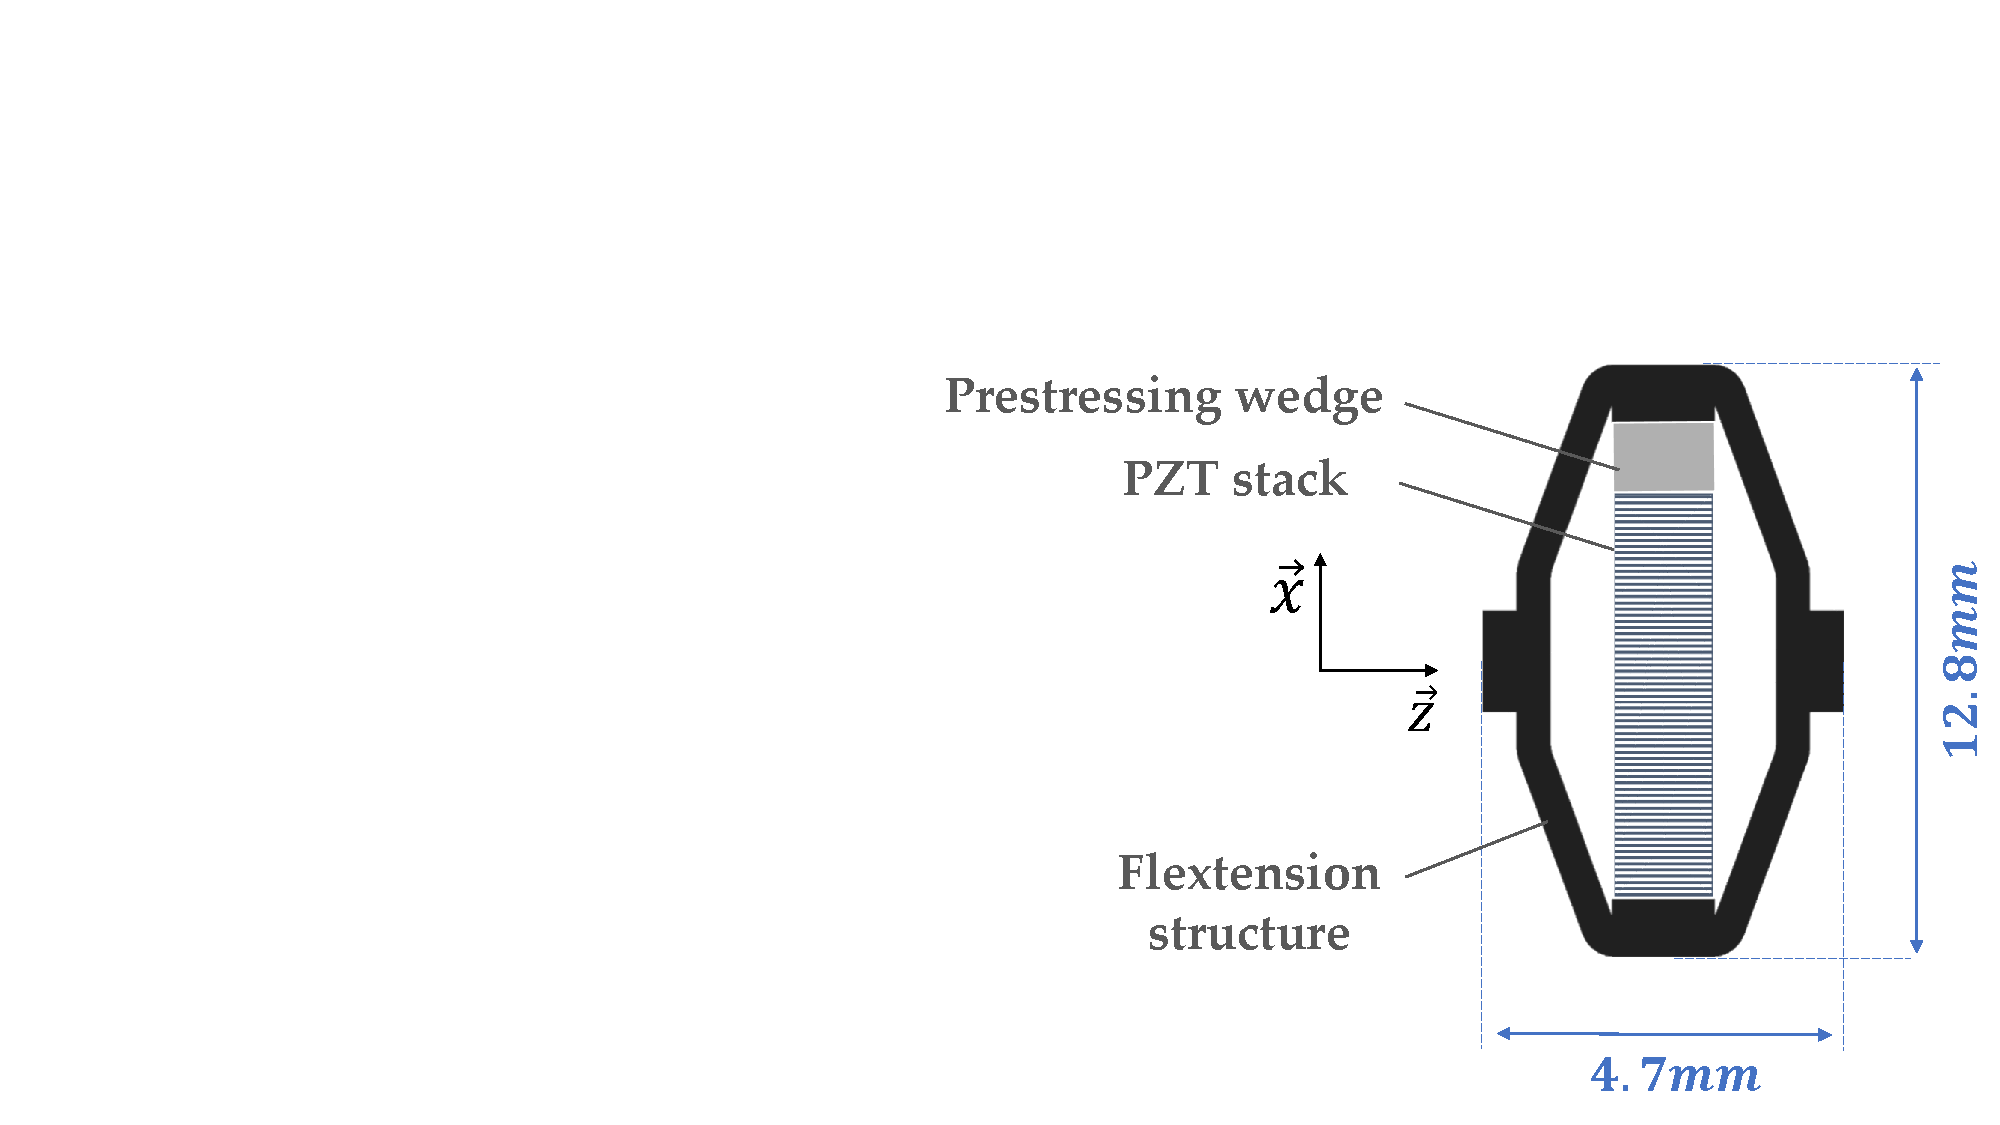
\includegraphics[trim={13cm 0cm 0cm 6cm},clip,width=\linewidth]{figures/APG_schema.pdf}
			\caption{Detailed schema}
			\label{fig:APG_schema}
		\end{subfigure}
		\hfillx
		\begin{subfigure}[t]{0.21\linewidth}
			\captionsetup{justification=centering}
			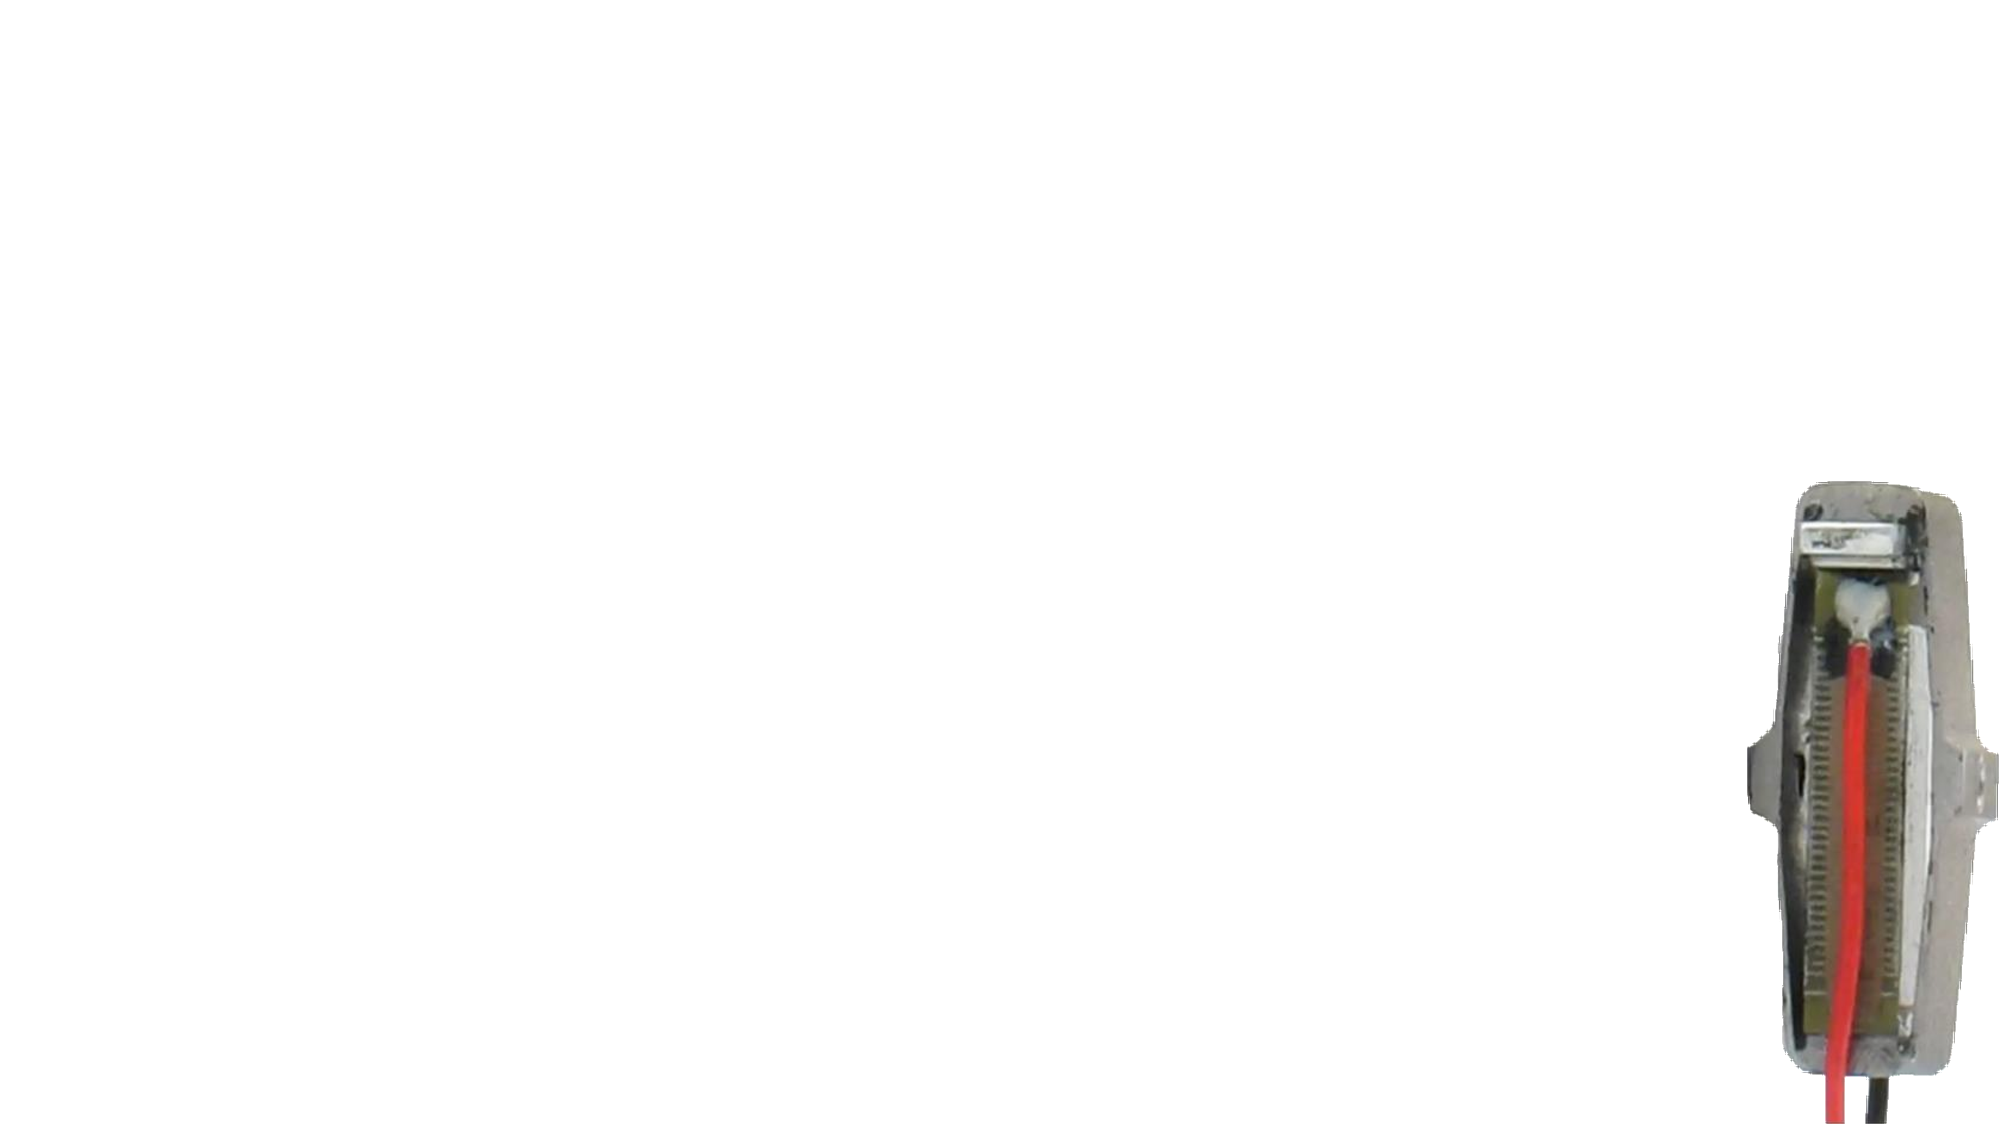
\includegraphics[trim={29.5cm 0cm 0cm 8cm},clip,width=0.65\linewidth]{figures/APG_photo.pdf}
			\caption{Picture}
			\label{fig:APG_photo}
		\end{subfigure}
		\caption{The APG presentation}
		\label{fig:APG}
	\end{center}
\end{figure}
%%%%%%%%%%%%%%%%%%%%%%%%%%%%%%%%%%%% 

The electromechanical converter is actuated, by two hydraulic cylinders (HC), with the hydraulic energy transmitted from the liquid filled earplug, through a hydraulic amplifier (HA) and two hydraulic valves (HV).

During a mastication cycle, the TMJ compresses the ear canal wall and expels the fluid out of the earplug. The HVs led the fluid alternatively to each HC in order to actuate the BR mass back and forth. The HA adapts both the cylinders stroke to the available earplug swept volume and the actuation force of the BR to the comfort pressure of the ear canal (fig. \ref{fig:system_presentation}).

The BR mass has two stable equilibrium positions, \mbox{$x_m = x_0$ }and \mbox{$-x_0$}. The harvester operates on two major phases. The first consists on the BR mass actuation, by a HC, from one stable equilibrium position toward the unstable position at $x_m = 0$. During the second phase the mass reaches and oscillates around the opposite stable equilibrium position until it stops, while a portion of the vibration energy is converted into electricity by the GPA. The mass will move backward when the next mastication will occur and complete the harvester cycle.
%%%%%%%%%%%%%%%%%%%%%%%%%%%%%%%%%%%%%%%
\begin{figure}[!htbp]
	\centering
	\captionsetup{justification=centering}
	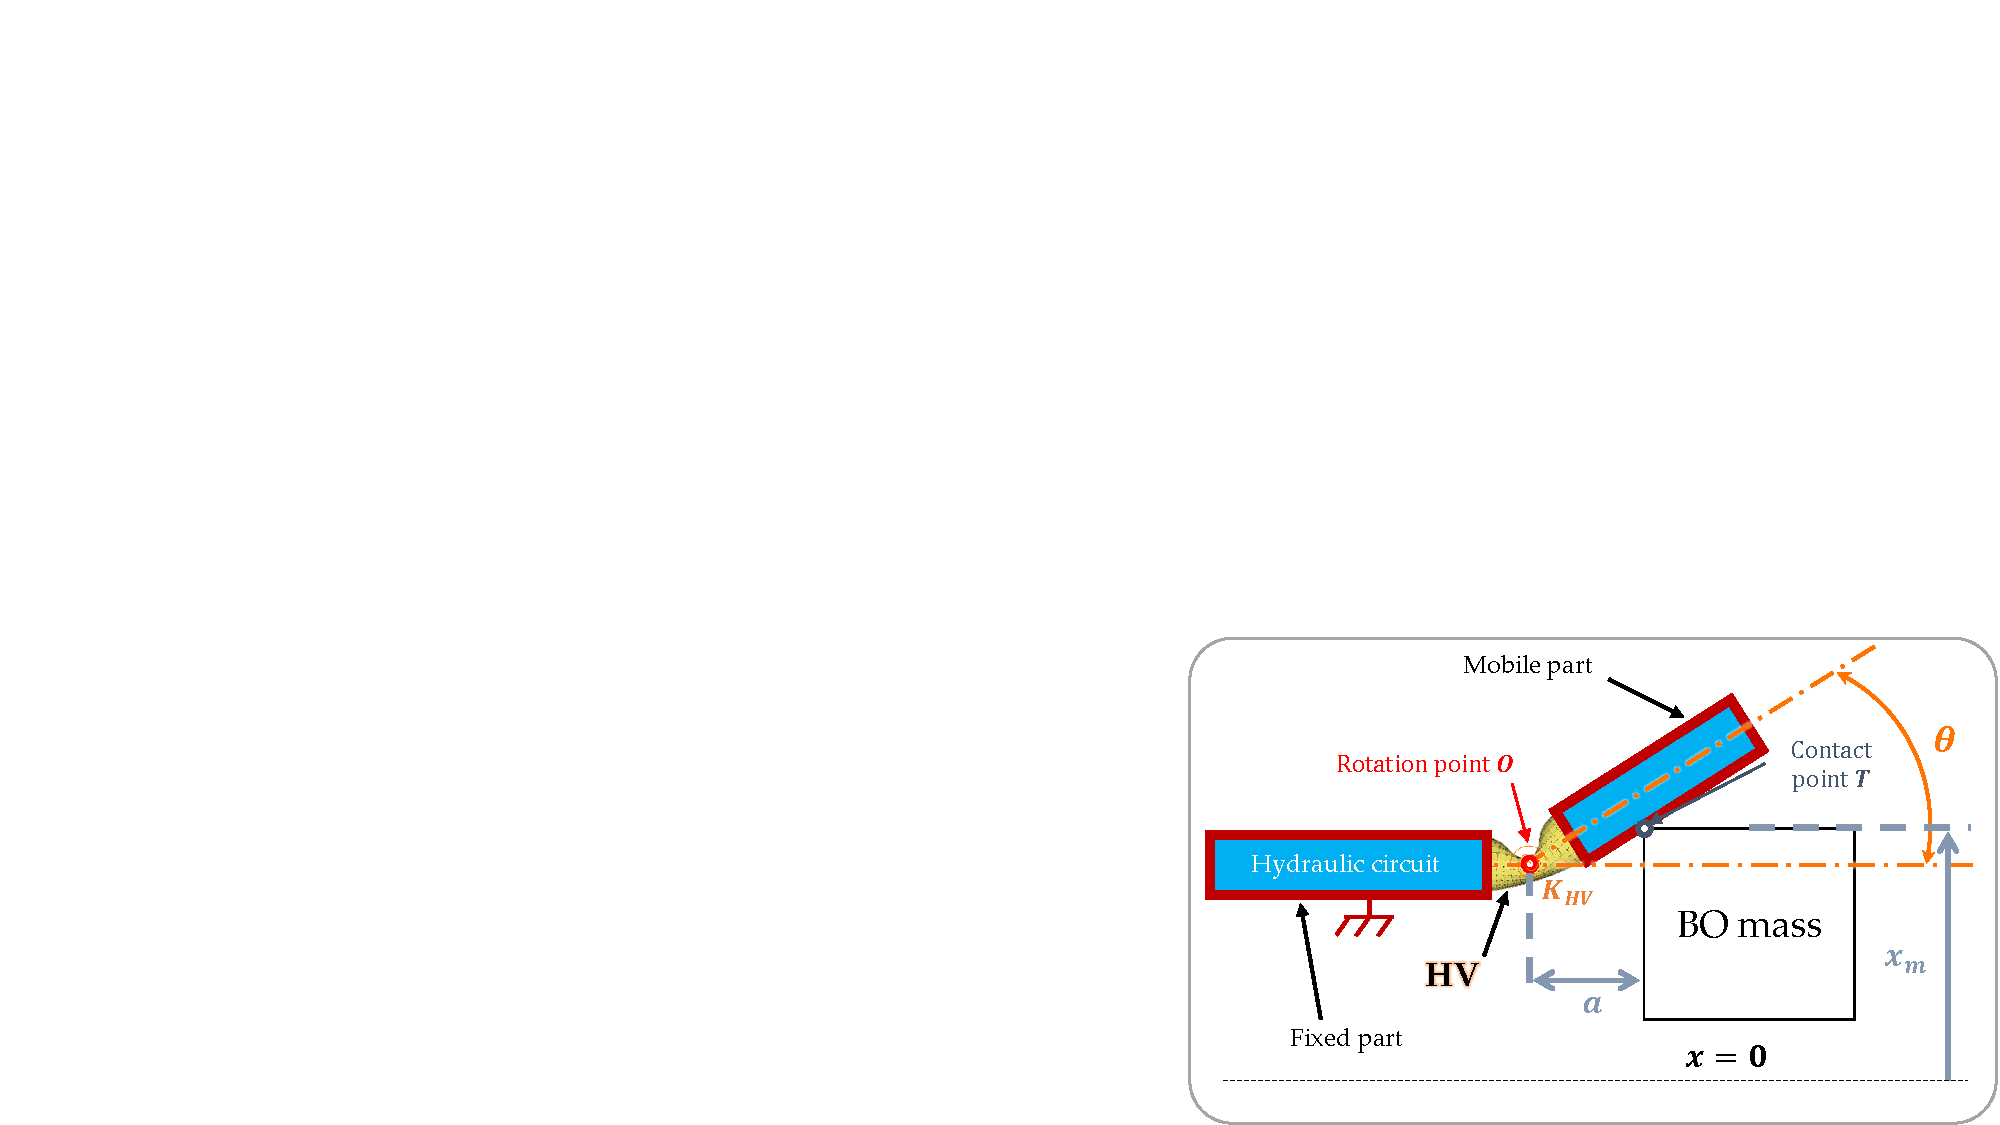
\includegraphics[trim={20.5cm 0cm 0cm 11.5cm},clip, width=0.8\linewidth]{figures/HV_actuation_detail.pdf}
	\caption{Contact detail between a HV and the BR mass} 
	\label{fig:HV_actuation_detail}
\end{figure}
%%%%%%%%%%%%%%%%%%%%%%%%%%%%%%%%%%%%%%%

A technological solution for the HV is to use a flexible tube buckled by bending. The figure \ref{fig:HV_actuation_detail} schematizes the integration of such a HV around the BR environment. The HV is composed of a flexible tube connected to the hydraulic circuit between a rigid mobile and rigid fixed sheaths. It is in contact with the mass at the T point. The mass motion on the mobile sheath induces a bending angle $\theta$ around the rotational point $O$ located at the buckled section of the flexible tube. Consequently, a pressure loss is generated through the valve in buckled position. The HV is to be closed when the BR mass is at a stable equilibrium position ($x_m=\pm x_0$) and opened when the mass is at $x_m=0$. This last point will be validated experimentally in section \ref{sec:EXPERIMENTAL APPROACH FOR THE HV DESIGN}. Two HVs symmetrically placed on each side of the $\vec{z}$ axis set up an opened hydraulic circuit on one side and a closed one on the other side, depending on the BR mass position. The HV technological choice is motivated by three major arguments. First, the absence of dedicated electromechanical transduction compared to a more usual actuated valve minimizes the energy losses for the valve operation. Then, the post-buckling softening effect of the bent tube minimizes the mechanical impact on the BR mass dynamic operation. Finally, it seems well adapted for integration purpose for millimetric application scale.

%/!\/!\/!\/!\/!\/!\/!\/!\/!\/!\/!\/!\/!\/!\/!\/!\/!\/!\/!\/!\/!\/!\/!\/!\%
\section{SYSTEM GLOBAL MODELING}
\label{sec:SYSTEM MODELING}
%/!\/!\/!\/!\/!\/!\/!\/!\/!\/!\/!\/!\/!\/!\/!\/!\/!\/!\/!\/!\/!\/!\/!\/!\%
This section presents the global multiphysic model describing the system operation. Two coupled subsystems are considered. The subsection \ref{subsec:The electromechanical converter} shows the modeling of the electromechanical frequency-up converter (BR + APG) under the mechanical influence of a HV and a HC. Subsection \ref{subsec:The hydraulic circuit} discusses the design of the hydraulic circuit composed of the two HVs, the two HCs, the hydraulic amplifier and the liquid filled earplug.

This work challenges are focused on the experimental validation of the electromechanical converter cycled by two hydraulic valves. In fact several hydraulic miniature solutions are introduced by the literature for both of the components \cite{Wang2020,Xu2021,Zhu2013}. Hence, this section neglects the pressure loss through the pressure separator and the energy loss inside the hydraulic amplifier. These hydraulic components will rather be considered for further work. 

    %///////////////////////////////////////////// 
	\subsection{Modeling of the electromechanical converter}	
	\label{subsec:The electromechanical converter}
    %/////////////////////////////////////////////
%%%%%%%%%%%%%%%%%%%%%%%%%%%%%%%%%%%%%%
\begin{figure*}[!htbp]
	\centering
	\captionsetup{justification=centering}
	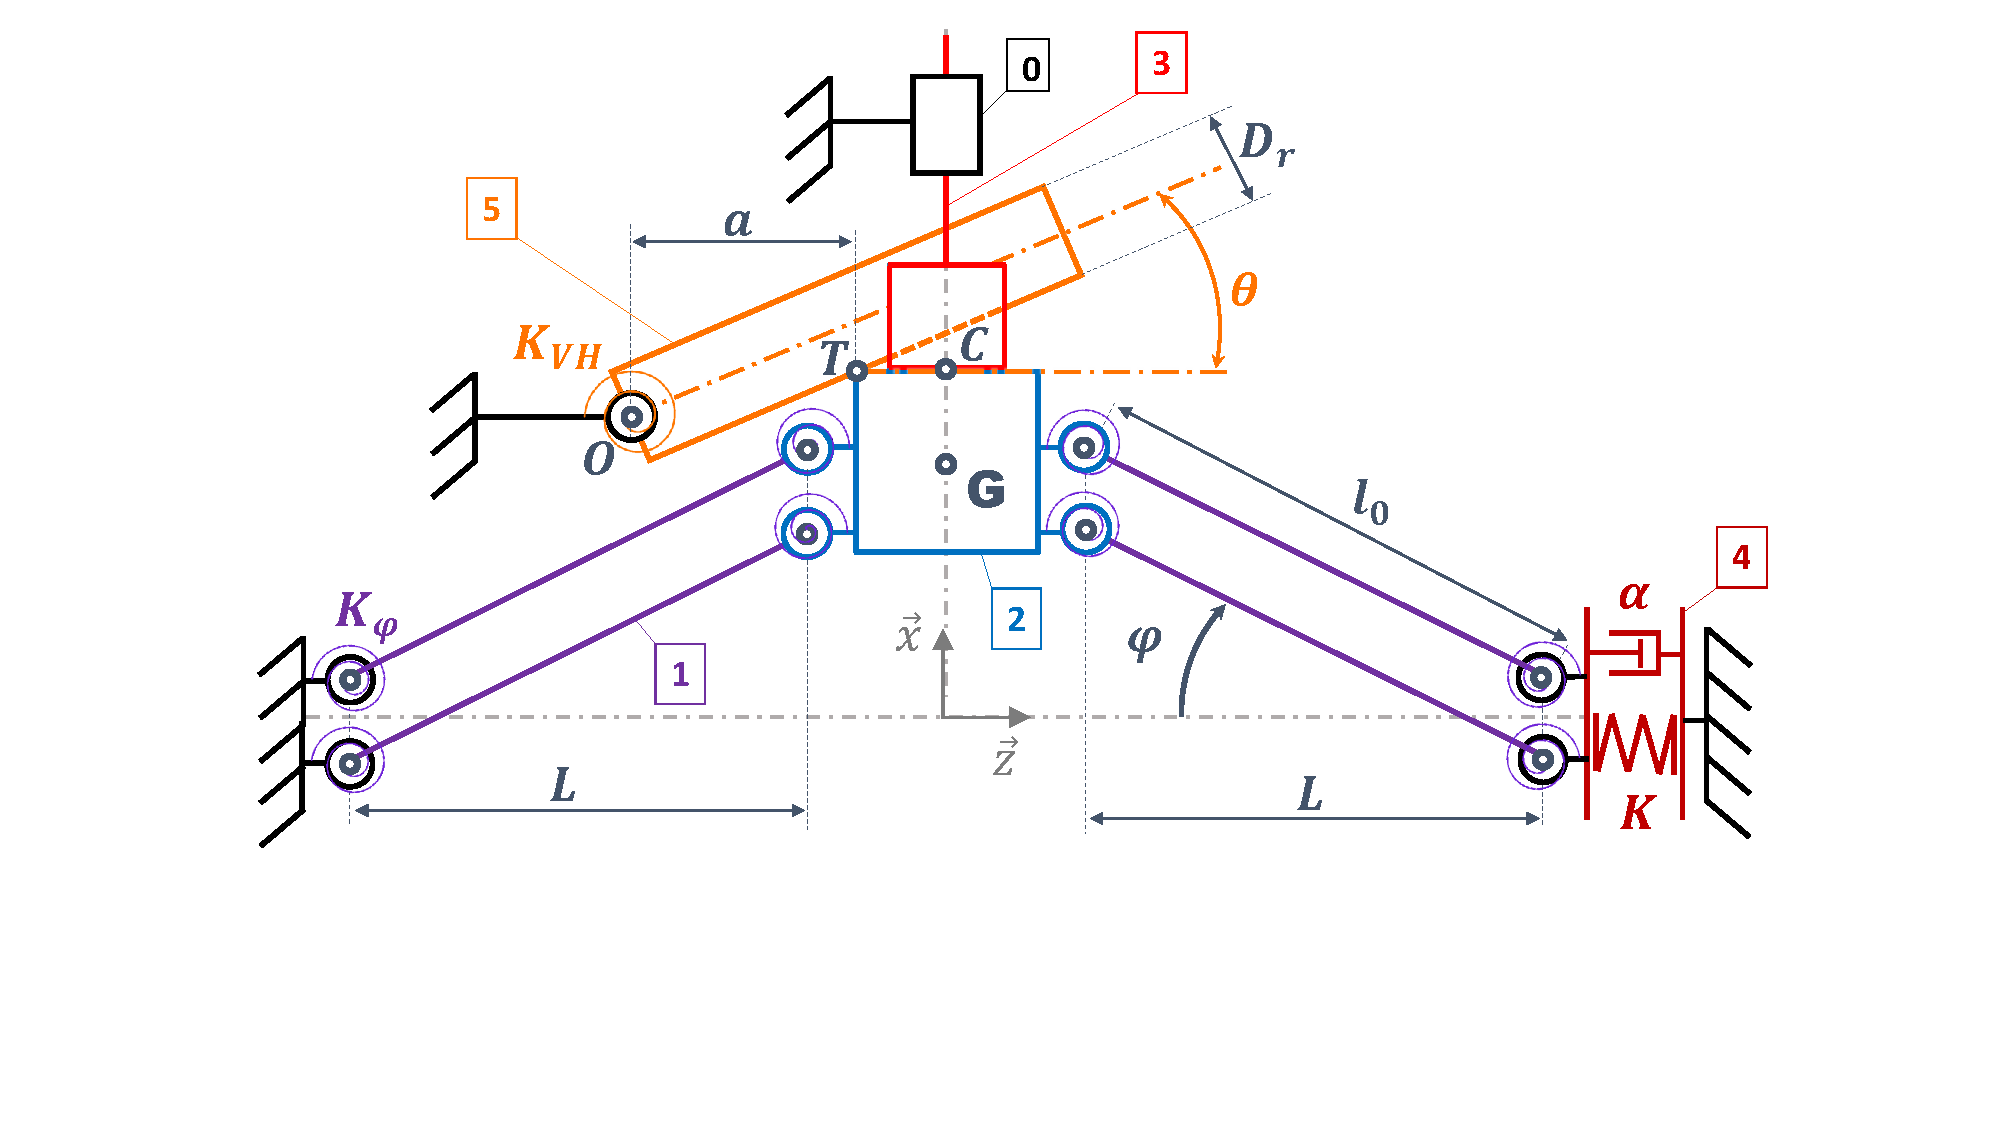
\includegraphics[trim={0cm 0cm 0cm 0cm},clip, width=0.9\textwidth]{figures/schema_cinematique1.pdf}
	\caption{Kinematic scheme of the electromechanical converter under the mechanical influence of a HV and a HC}
	\label{fig:schema_cinematique1}
\end{figure*}
%%%%%%%%%%%%%%%%%%%%%%%%%%%%%%%%%%%%%%

The figure \ref{fig:schema_cinematique1} shows the kinematic scheme of the electromechanical converter under the mechanical influence of a HV and a HC. The rigid bodies are defined in the table \ref{tab:Designation of rigid bodies}. The BR is represented by 4 identical arms articulated by 8 hinges and a central mass. The APG is considered as a spring of stiffness $K$ with an electromechanical coupling $k^2$, standing for the piezoelectric transduction and defined by the equation \ref{eq:k2_def}.\\
The model is based on the following hypotheses:
\begin{itemize}
	\item The only mass considered is the BR mass (2).
	\item All parts are rigid except for the APG (4).
	\item The hinges are considered elastic: They are defined by their rotational stiffness $K_{\varphi}$
	\item The mechanical damping of the hinges is included in the global viscous damping coefficient $\mu$.
	\item The contact between the BR mass (2) and the HC piston head (5) is considered permanent for $0 < x < x_0$.
	\item \mbox{$x_0 \ll L$}. 
\end{itemize}
\begin{equation}
	k^2 = \dfrac{\alpha^2}{\alpha^2 +  K C_p}
	\label{eq:k2_def}
\end{equation}
%%%%%%%%%%%%%%%%%
\begin{table}[!htbp]
\centering
\resizebox{0.6\linewidth}{!}{%
	\begin{tabular}{ c | c }
		\toprule
		\multicolumn{1}{c}{\textbf{Num}} &
		\multicolumn{1}{c}{\textbf{Name}}                                 \\
		\midrule
		0                                & Fixed frame                    \\
		1                                & BR arm                         \\
		2                                & BR mass                        \\
		3                                & HC piston head                 \\
		4                                & APG                            \\
		5                                & Simplified HV mechanical model \\
		\bottomrule
	\end{tabular}}
\caption{Definition of figure \ref{fig:schema_cinematique1} bodies}
\label{tab:Designation of rigid bodies}
\end{table}
%%%%%%%%%%%%%%%%%%%%%  

By isolating the BR mass and using the Newtons 2$^{nd}$ law, we can express its dynamic equilibrium. The projection on the $\vec{x}$ axis of the resulting expression is given by the equation \ref{eq:OB-GPA}. The BR mechanical equilibrium has a mass inertial term, a non-linear stiffness depending on $x_m$, the stiffness of the hinge $K_{\varphi}$ and viscous losses. The first term introduced by the HV is related to its rotational stiffness $K_{HV}$ and the second term is related to the friction losses at the contact point $T$ (fig. \ref{fig:HV_actuation_detail}). $K_{HV}$ and $K_{\varphi}$ both act the same way by shifting the stable equilibrium positions of the BR toward $0$ as much as they increase. A dry friction model is chosen to describe the dissipation effect of the contact. The rubbing efforts depend on a dry friction coefficient $f_d$, related to the nature of the material that are rubbing, and the sign of $\dot{x}_m$. The coefficient $\mu_{hc}$ models the viscous friction at the sealing gasket of the HC. The hydro-mechanical coupling will be detailed later.

The electrical power generated by the APG is dissipated in a load resistor $R_l$ calculated with an adaptive impedance matching expressed in the equation \ref{eq:R_ch_adaptive_imp} \cite{Liu2013}. 
\begin{equation}
	R_l = \dfrac{1}{C_p w_0}
	\label{eq:R_ch_adaptive_imp}
\end{equation}
Thus, the electrical equation of the APG is :
\begin{equation}
	\dfrac{U_p}{R_l} = 
	-\alpha\dfrac{d}{dt}\biggl(2\sqrt{{l_0}^2-x_m^2}\biggr)
	- C_p\dot{U_p}
	= \frac{2\alpha x_m\dot{x}_m}{\sqrt{L^2+x_m^2}} - C_p\dot{U_p}
	\label{eq:APG_elec}
\end{equation}
Consequently, the generated power $P_e$ is :
\begin{equation}
	P_e = \frac{{U_p}^2}{R_l} 
	\label{eq:P_e}
\end{equation} 
Equation \ref{eq:theta_fonction_de_xm} defines the implicit relation between $\theta$, $x_m$ and the geometrical parameters of the setup. Where the hinges angle $\varphi$ is defined as :
\begin{equation}
	\varphi = \arctan\biggl(\dfrac{x_m}{L}\biggr)
	\label{eq:phi_definition}
\end{equation}
Additionally, the HV stiffness $K_{HV}$ will depend on its bending angle $\theta$, as showed in figure \ref{fig:HV_actuation_detail}. 
%%%%%%%%%%%%%%%%%%%%%%%
\begin{figure*}[!htb]
\begin{equation}
 m \ddot{x}_m =-2K_{eq}(\sqrt{x_m^2+L^2}-l_0)\tan(\varphi(x_m)) -\mu \dot{x}_m -\frac{4K_{\varphi}\varphi}{L}
				\ -2\alpha U_p \tan(\varphi(x_m))
				\ -\dfrac{K_{HV}(x_m)\theta(x_m)}{a} - f_d \text{sign}(\dot{x}_m)
				\  - p_{hc,a}\ S_{hc} - \mu_{c}\ \dot{x}_m
\label{eq:OB-GPA}
\end{equation}
\end{figure*}
% \FloatBarrier
%%%%%%%%%%%%%%%%%%%%%%%
%%%%%%%%%%%%%%%%%%%%%%%
\begin{equation}
\resizebox{.9\linewidth}{!}{$	
x_m = \Biggl[ \dfrac{D_r(1-\cos(\theta))+2a\sin(\theta)}{2\cos(\theta)}\text{,}
				~~ \theta\leq\arctan\biggl(\dfrac{2a}{D_r}\biggr) \Biggr]
				$}
\label{eq:theta_fonction_de_xm}
\end{equation}
%%%%%%%%%%%%%%%%%%%%%%%
% %%%%%%%%%%%%%%%%%%%%%%%
% \begin{figure*}
% \begin{equation}
% % \begin{small}
% 	\begin{dcases}
% \ddot{x}_m = - \frac{2K{x_0}^2}{mL^2}\Biggl[\biggl(\frac{x_m^2}{{x_0}^2} -1\biggr )+ \dfrac{8K_{\varphi}}{L^2}\Biggr]x_m 
% 			 - \frac{K_{HV}(x_m)\theta(x_m)}{ma}
% 			 - \frac{\mu+\mu_{hc}}{m}\dot{x}_m  - f_d \text{sign}(\dot{x}_m)
% 			 - \frac{2\alpha U_p\ x_m}{mL}
% 			 - p_{hc,a}\ S_{hc} \\
% x_m = \dfrac{D_r(1-\cos(\theta))+2a\sin(\theta)}{2\cos(\theta)}\text{,}
% 				~~ \theta\leq\arctan\biggl(\dfrac{2a}{D_r}\biggr)\\
% \dfrac{U_p}{R_l} = \frac{2\alpha x_m \dot{x}_m}{L} - C_p\dot{U}_p 
% 	\end{dcases}
% 	\label{eq:OB+GPA+VH+piston}	
% % \end{small}
% \end{equation}
% \end{figure*}
% % \FloatBarrier
% %%%%%%%%%%%%%%%%%%%%%%%
    %///////////////////////////////////////////// 
	\subsection{Modeling of the hydraulic circuit}	
	\label{subsec:The hydraulic circuit}
    %/////////////////////////////////////////////

In order to model the coupled behavior of the two hydraulic branches, we will use the index "$a$" for the active branch where the fluid flows and the index "$i$" for the inactive one. \\
The following hypotheses will be considered :
\begin{itemize}
	\item The flow is incompressible and Newtonian.
	\item The hydraulic circuit is rigid (no volume change) and there is no leakage.
	\item The hydraulic actuation is considered quasi-static considering the oscillation frequency of the BR.
\end{itemize}
The mechanical equilibrium is :
\begin{align}
	\text{Inactive cylinder ~}& \left\{~
	p_{hc,i}\ S_{hc} - \mu_{c}\ \dot{x}_{hc,i} = 0
	\right.
	\label{eq:equilibre_dynamique_piston_ferme}
\end{align}
The pressure loss coefficient $Cf$ for a buckled flexible tube will depend on the HV bending angle $\theta$ and therefore on the BR mass position $x_m$ (fig. \ref{fig:HV_actuation_detail}). $Cf$ will be all the more important as $x_m$ increases. Its minimal value $Cf_0$ is obtained when the HV is unbent. We preliminarily assume that the relationship between $Cf$ and $x_m$ is linear and defined as follows :
\begin{align}
Cf(x_m) & = Cf_0 + \dfrac{Cf_c - Cf_0}{x_0}\ |x_m| 
\label{eq:Cf(x_m)_linear}
\end{align}
Where $Cf_c=Cf(\pm x_0)$. Regarding the BR symmetry, the relation between $Cf$ and $x_m$ has to be an even function to allow the system cycling, i.e. $Cf(x_m) = Cf(-x_m)$.

Using the Bernoulli's equation for a current line, we can express the earplug inside pressure $p_{ear}$ as a function of the hydraulic resistance in the two parallel branches with the equations \ref{eq:Bernoulli_piston_ouvert} and \ref{eq:Bernoulli_piston_ferme}.
\begin{align}
	\text{Active branch ~}& \left\{~
	p_{ear} = \dfrac{1}{a_h}\biggl(p_{hc,a} + Cf_0 {q_a}^2 \biggr)
	\right.
	\label{eq:Bernoulli_piston_ouvert}\\
	\text{Inactive branch ~}& \left\{~
	p_{ear} = \dfrac{1}{a_h}\biggl(p_{hc,i} + Cf(x_m) {q_i}^2 \biggr)
	\right.
	\label{eq:Bernoulli_piston_ferme}
\end{align}
Where $a_h$ is the hydraulic amplification ratio and $q$ the fluid flow rate.

The no leakage assumption imposes that all the fluid exiting the earplug is contained in the two hydraulic branches (eq. \ref{eq:conservation_masse}).
\begin{equation}
	q_{ear} = \dot{\Delta V_{ear}} = q_a + q_i
	\label{eq:conservation_masse}
\end{equation}
Moreover, the fluid entering the HC necessarily results on a piston displacement (eqs. \ref{eq:conservation_masse_ouvert},\ref{eq:conservation_masse_ferme}).
\begin{align}
	\text{Active cylinder ~}& \left\{~
	q_a = S_{hc} \dot{x}_m
	\right.
	\label{eq:conservation_masse_ouvert}\\
	\text{Inactive cylinder ~}& \left\{~
	q_i = S_{hc} \dot{x}_{ic}
	\right.
	\label{eq:conservation_masse_ferme}
\end{align}
%/!\/!\/!\/!\/!\/!\/!\/!\/!\/!\/!\/!\/!\/!\/!\/!\/!\/!\/!\/!\/!\/!\/!\/!\%
\section{NUMERICAL MODEL AND SIMULATIONS}
\label{sec:NUMERICAL MODEL AND SIMULATIONS}
%/!\/!\/!\/!\/!\/!\/!\/!\/!\/!\/!\/!\/!\/!\/!\/!\/!\/!\/!\/!\/!\/!\/!\/!\%
    %///////////////////////////////////////////// 
	\subsection{The harvester parameters setting}	
	\label{subsec:The harvester setting}
    %/////////////////////////////////////////////
The energy system combines many variable parameters. In order to determine them, it is first necessary to identify the fixed technological elements: 
\begin{itemize}
	\item The transducer is a APA50XS piezoelectric actuator, from Cedrat Technologies, exploited as a generator \cite{CEDRATTECHNOLOGIES2022}.
	\item The hydraulic actuation is ensured by the SMC MQP4-10S HCs which allow a 1kPa pressure operation \cite{SMC2022}.
	\item The usual hearing aid size is $50$x$20$x$10$mm \cite{Quattro2019}. The \mbox{$L=16mm$} parameter is chosen to be consistent with this scale.
\end{itemize}

The system is designed by setting the two coupled requirements allowing the system operation. First, the available swept volume must be enough to ensure the HC stroke from its equilibrium position until the BR mass reaches \mbox{$x_m=0$} (eq. \ref{eq:contrainte_course}). Then, the BR mechanical force on $\vec{x}$ axis reaches a maximum value $F_c$ when \mbox{$ x_m = x_c = \dfrac{x_0}{\sqrt{3}}$}. At this point, a maximum pressure is induced in the earplug and so the equation \ref{eq:contrainte_confort} has to be verified to guarantee the pressure limit. If not, $\epsilon$ (éq. \ref{eq:epsilon_def}) can be decreased, diminishing the extracted energy.
\begin{empheq}[left=\empheqlbrace]{align} 
	(\Delta V_{ear})_{max} = a_h\ S_{hc}\  x_{c0}
	\label{eq:contrainte_course}\\
	p_c > \frac{1}{a_h} \frac{F_c}{S_{hc}} ~~~~ \text{with}~~~~ F_c = \dfrac{4Kx_0\epsilon}{3\sqrt{3}}
	\label{eq:contrainte_confort}
\end{empheq}
\begin{equation}
	\epsilon = \dfrac{x_0}{L}
	\label{eq:epsilon_def}
\end{equation}
Equations \ref{eq:contrainte_course} and \ref{eq:contrainte_confort} set the amplification level $a_h$ and the BR buckling level $\epsilon$. Regarding the technological choices and the system operation requirements, we can evaluate $n=65\%$. This value can be compared to the best theoretical linear energy extraction solution described in \ref{eq:best_linear_soution}.
	%///////////////////////////////////////////// 
	\subsection{Targeted hydraulic behavior of the HVs}	
	\label{subsec:HV hydraulic targeted behavior}
	%/////////////////////////////////////////////
A multiphysic coupled model has been established with the equations and the preliminary dimensioning previously introduced. 
The unknown remaining key parameter stays the hydraulic behavior $Cf(x_m)$ of the HVs. 
The ratio between the pressure loss coefficient of the closed HV and the one of the opened HV has to be sufficient to force the flow through the opened branch. 
So we introduce the hydraulic restriction coefficient $r_{Cf}$ defined as follows :
\begin{equation}
	r_{Cf} = \dfrac{Cf(\text{Closed HV})}{Cf(\text{Opened HV})}	= \dfrac{Cf_c}{Cf_0}	
	\label{eq:r_Cf_definition}
\end{equation}
The numerical resolution of the coupled differential equations \ref{eq:APG_elec},\ref{eq:OB-GPA}, \ref{eq:equilibre_dynamique_piston_ferme}, \ref{eq:Bernoulli_piston_ouvert}, \ref{eq:Bernoulli_piston_ferme}, \ref{eq:conservation_masse}, \ref{eq:conservation_masse_ouvert} and \ref{eq:conservation_masse_ferme} can provide the minimum value $(r_{Cf})_{min}$ to reach in order to perform the adequate hydraulic commutation.
	%///////////////////////////////////////////// 
	\subsection{Simulation results}	
	\label{subsec:Simulation results}
	%/////////////////////////////////////////////
By imposing a volume variation $\Delta V_{ear}(t)$ recorded during the mastication cycle of a human subject (fig. \ref{fig:deltaV_ear}), the numerical model gives the theoretical temporal evolution of the hydraulic, mechanic and electric coupled variables defining the harvester. The earplug is assumed to be a perfect flow rate source. The mastication cycle is identically used 4 times in order to test the system cycling robustness. The fixed, designed and resulting theoretical parameters of the simulated global model are presented in tables \ref{tab:parametres électromécaniques} and \ref{tab:parametres_hydrauliques}.

Figure \ref{fig:positions+DeltaV_debits_pear} shows the simulation results of the mass and the HC pistons positions over overlaid with $\Delta V_{ear}(t)$, the flow rates in the two parallel branches and the earplug pressure. The two different sides are identified on the curves by the indexes $t$ for \emph{"top"} side ($x>0$) and $b$ for \emph{"bottom"} side ($x<0$), noting that the gravity influence is not considered. The same figure shows a focused view on the two main phases of the harvester operation during the actuation by the \emph{"bottom"} HC. The simulation begins with the following initial conditions:
\begin{itemize}
	\item The mass is at the \emph{"bottom"} equilibrium position $-x_0$.
	\item The \emph{"top"} HV is closed ($Cf_{top} = Cf_c$) and the \emph{"bottom"} side HV is opened ($Cf_{bot} = Cf_0$).
	\item There is no contact between the mass and the HCs.
	\item A mastication occurs.
\end{itemize}

During a first phase the BR mass is pushed until it reaches $x=0$. The fluid exiting the earplug is mostly guided toward the \emph{"bottom"} HC and a pressure is induced in the earplug by the BR counter-reaction force. The mass then crosses $x_m=0$ and the second phase begins. The \emph{"top"} HV then opens ($Cf_{top} = Cf_0$) and the \emph{"bottom"} side HV closes ($Cf_{bot} = Cf(x_m)>Cf_0$). The fluid is then directed toward the \emph{"top"} side and there is no contact between the mass and a HC. The mass oscillates around $x_m=x_0$ and energy is harvested by the APG. The adequate hydraulic actuation making the fluid flow toward the right HC is achievable when \mbox{$(r_{Cf})_{min}=26$}. 

Additionally, figure \ref{fig:positions_Up_puissances_energies} presents the APG voltage, the source and harvested powers and the different energies entering and exciting the system. The theoretical global efficiency of the harvester is evaluated at \mbox{$\eta_g=76$\%} with $22$µJ electrical energy harvested from one mastication. The energy losses are mostly located in the BR stage and depend on the quality factor $Q$ that has been set in accordance with previous work results on similar BR architectures \cite{Liu2013}. The energy source is limited by the comfort pressure level $p_c$ that is set to 1kPa, i.e. a fraction of the theoretical maximal value of $12$kPa \cite{Bouchard-Roy2020}. The harvester theoretical efficiency could lead to a maximum of $684$µJ extractable from the ear canal.

%%%%%%%%%%%%%%%%%%%%%%%%%%%%%%%%%%%%%%
\begin{figure*}[!htbp]
	\centering
	\captionsetup{justification=centering}
	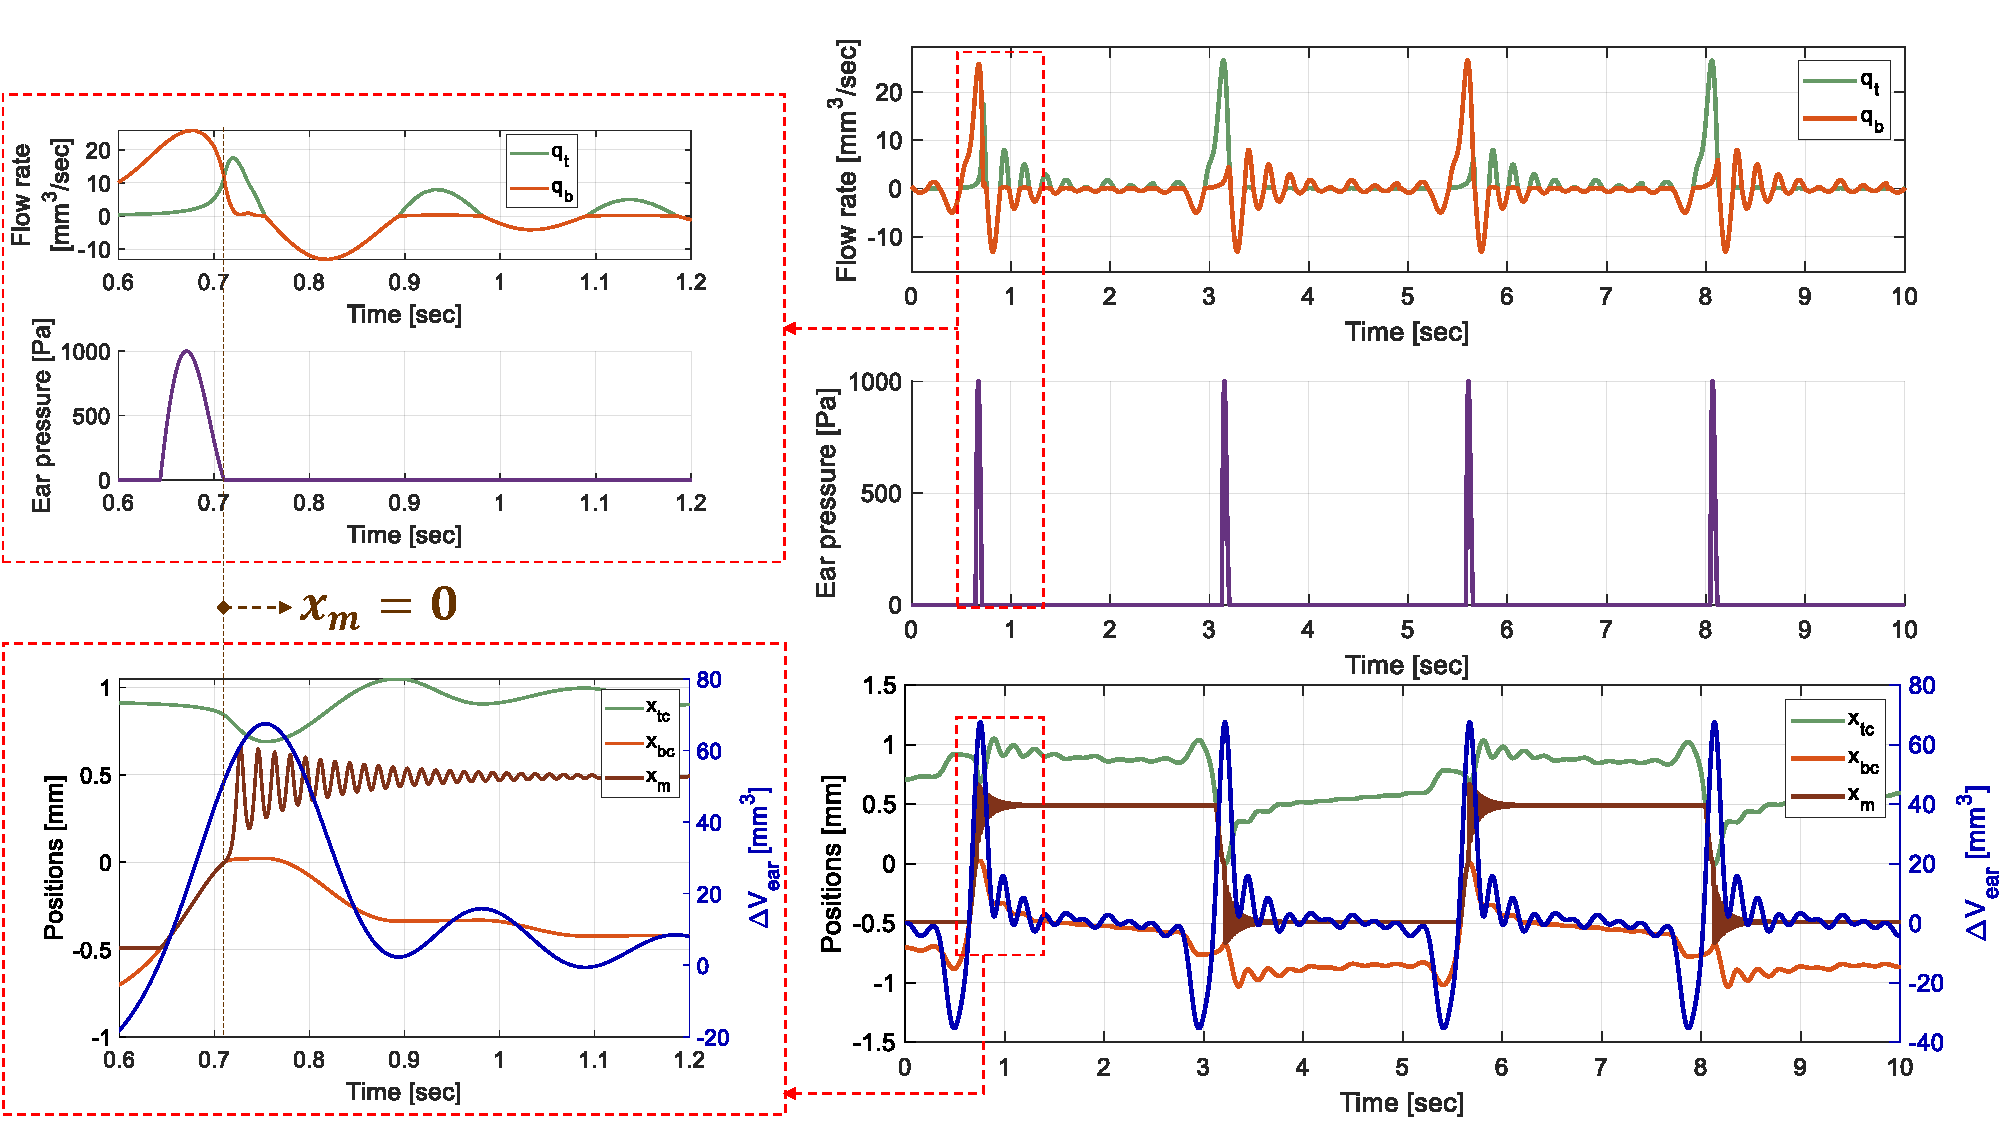
\includegraphics[trim={0cm 0cm 0cm 0.5cm},clip, width=\textwidth]{figures/positions+DeltaV_debits_pear.pdf}
	\caption{}
	\label{fig:positions+DeltaV_debits_pear}
\end{figure*}
%%%%%%%%%%%%%%%%%%%%%%%%%%%%%%%%%%%%%%%
%%%%%%%%%%%%%%%%%%%%%%%%%%%%%%%%%%%%%%
\begin{figure*}[!htbp]
	\centering
	\captionsetup{justification=centering}
	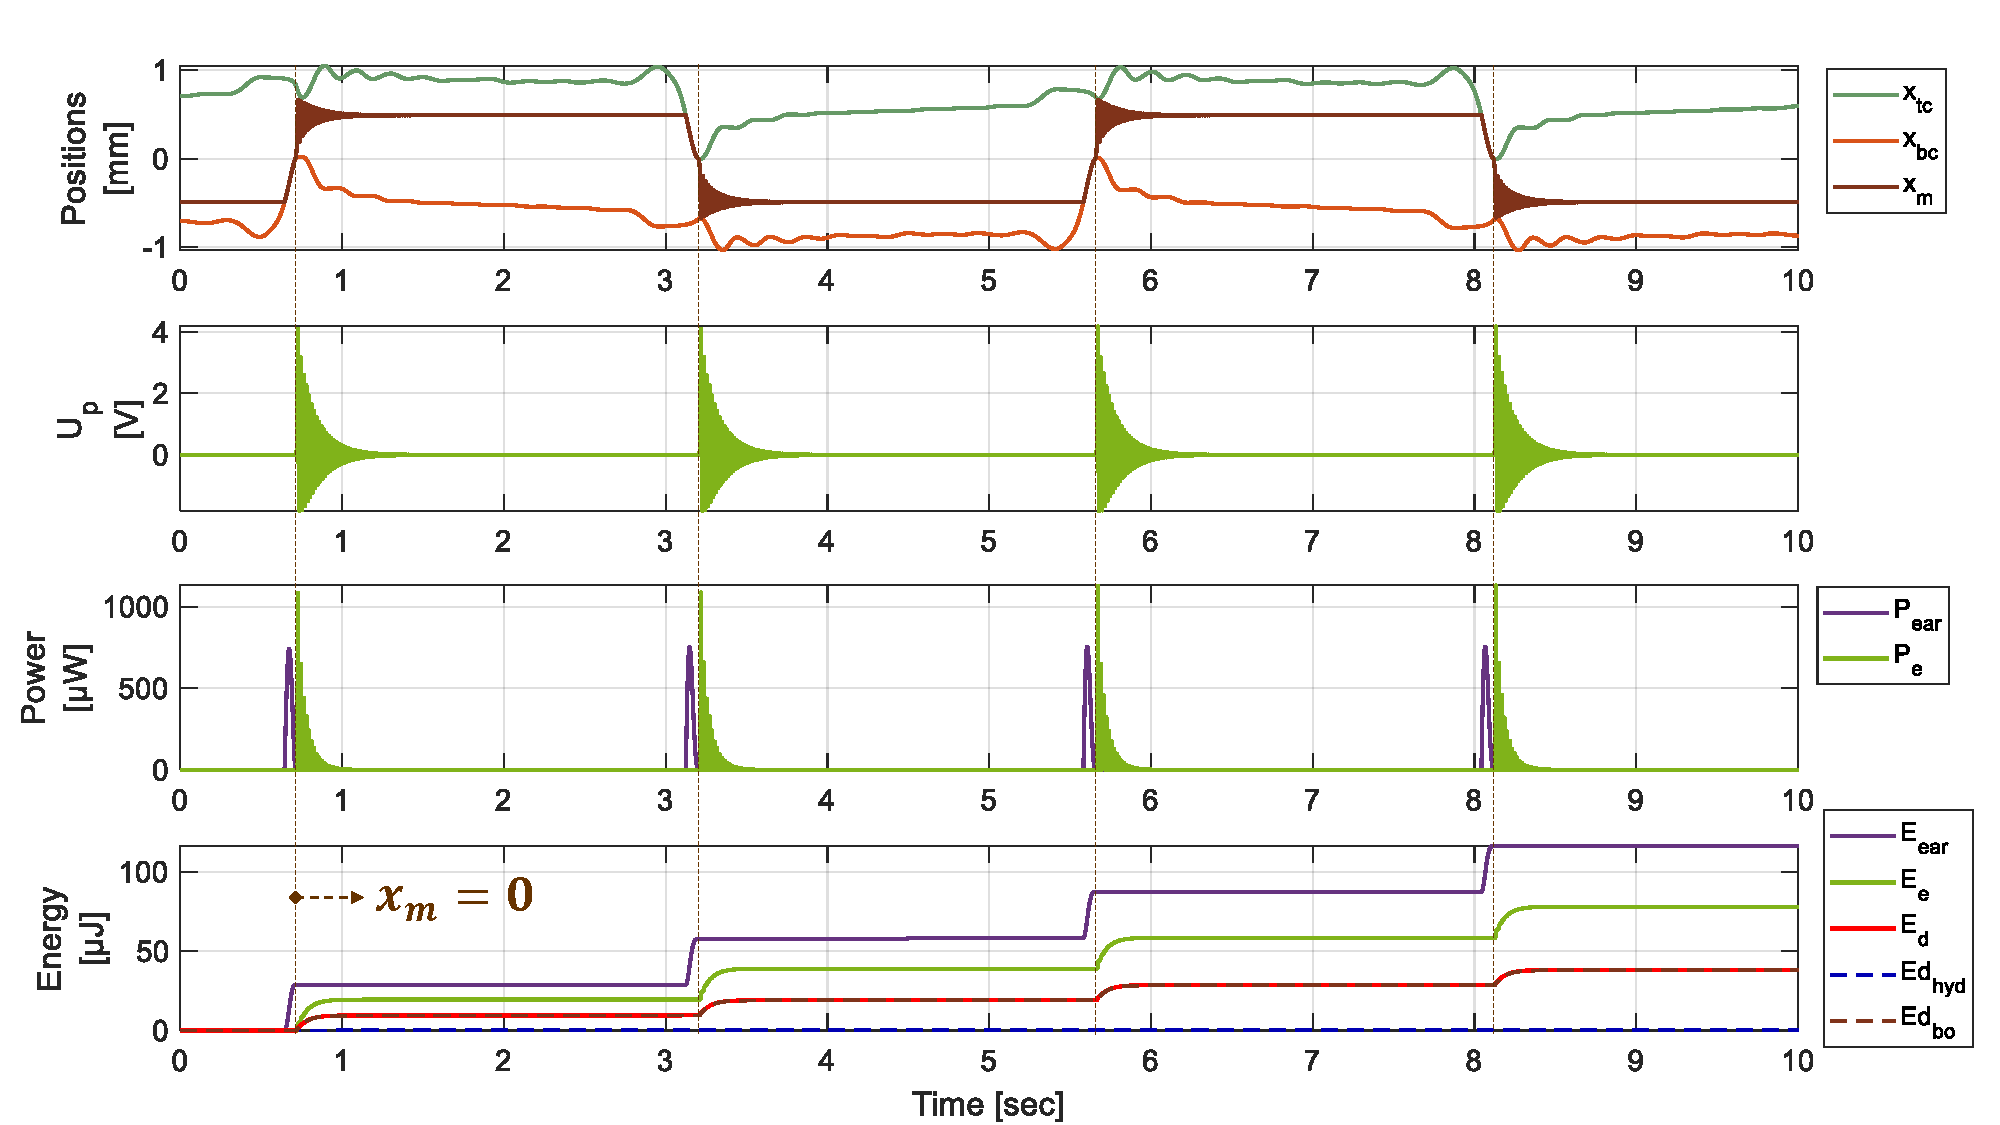
\includegraphics[trim={0cm 0cm 0cm 0cm},clip, width=\textwidth]{figures/positions_Up_puissances_energies.pdf}
	\caption{}
	\label{fig:positions_Up_puissances_energies}
\end{figure*}
%%%%%%%%%%%%%%%%%%%%%%%%%%%%%%%%%%%%%%%
%%%%%%%%%%%%%%%%%%%%%%%%%%%%%%%%%	
\begin{table}
\begin{subtable}[b]{.42\linewidth}
	\centering
	\resizebox{\linewidth}{!}{%
	\begin{tabular}{c|c}
\toprule
\multicolumn{1}{c}{~~\textbf{Parameter}~~}  & \multicolumn{1}{c}{~~\textbf{Value}~~} \\
\midrule
$K$	[N/µm]		&	0.256		\\	\hline
$x_0$ [mm]			&	0.49		\\	\hline
$L$	[mm]			&	16.0		\\	\hline
$m$	[g]				&	5.88		\\	\hline
$x_{c0}$ [mm]		&	0.69		\\	\hline
$R_l$ [k$\Omega$] 	&	6.39		\\	\hline
$\alpha$ [N/V]		&   0.105		\\	\hline
$C_p$ [µF]	   		&	0.25		\\	\hline
$Q$ [-]				&	50			\\	\hline
$\eta_g$ [\%]		& 	76			\\
\bottomrule
	\end{tabular}}
	\caption{Electromechanical}
	\label{tab:parametres électromécaniques}			
\end{subtable}
\hfillx
\begin{subtable}[b]{.55\linewidth}
	\centering
	\resizebox{\linewidth}{!}{%
	\begin{tabular}{c|c}
\toprule
\multicolumn{1}{c}{~~\textbf{Parameter}~~}  & \multicolumn{1}{c}{~~\textbf{Value}~~} \\
\midrule
$D_{hc}$ [mm] 	   			&	4						\\ \hline
$a_h$ [-]					&	29			 			\\ \hline
$p_c$ [kPa]					&	1				 		\\ \hline
$(\Delta V{ear})_{max}$ [mm$^3$]	& 60				\\ \hline
$Cf_0$ [Pa.s$^2$/m$^6$]			&	0.21e17			\\ \hline
$r_{Cf}$ [-]						&	26				\\ 
\bottomrule 
	\end{tabular}}
	\caption{Hydraulic}
	\label{tab:parametres_hydrauliques}		
\end{subtable}
\caption{Simulated model theoretical parameters}
\end{table}
%%%%%%%%%%%%%%%%%%%%%%%%%%%%%%%%%

The simulated model shows promising efficiency (tab. \ref{tab:parametres électromécaniques}) and demonstrates that a minimum value of 26 is required on the hydraulic restriction coefficient (tab. \ref{tab:parametres_hydrauliques}) to ensure the adequate cycled actuation of the BR mass. Next section will present the experimental approach to validate the theoretical behavior of the electromechanical converter.

%/!\/!\/!\/!\/!\/!\/!\/!\/!\/!\/!\/!\/!\/!\/!\/!\/!\/!\/!\/!\/!\/!\/!\/!\%
\section{EXPERIMENTAL CHARACTERIZATION OF THE \mbox{ELECTROMECHANICAL} CONVERTER}
\label{sec:EXPERIMENTAL CHARACTERIZATIONS OF THE ELECTROMECHANICAL CONVERTER}
%/!\/!\/!\/!\/!\/!\/!\/!\/!\/!\/!\/!\/!\/!\/!\/!\/!\/!\/!\/!\/!\/!\/!\/!\%
    %///////////////////////////////////////////// 
	\subsection{The electromechanical converter presentation}	
	\label{The electromechanical converter presentation}
    %/////////////////////////////////////////////
The BR is fabricated by electrical discharge machining (EDM) in a monobloc structure. This method optimizes the resonator quality factor by avoiding assemblies. Figure \ref{fig:BDT_OB+GPA} shows the BR mounted on the experimental test bench. The 8 hinges are realized by 4 buckled blades (BB) while a vertical guide beam (GB) ensures the APG mounting and avoids any of its rotations. The local thickenings at the midspan of the blades are intended to facilitate the fabrication. They also maximize the BB compression stiffness that maximizes harvester efficiency, as detailed in the following section. The geometrical and mechanical parameters of the BR are referenced in table \ref{tab:parametres_lames}. The following sections describe the design method that led to the dimensions of the blades that depend on our needs.
%%%%%%%%%%%%%%%%%
\begin{table}[!htbp]
	\centering
    \resizebox{\linewidth}{!}{%
		\begin{tabular}{l|c|c}
			\toprule
\textbf{Parameter definition} & \textbf{Symbol}    & \textbf{Valeur [Unit]} \\
\midrule
APX4 steel Young's modulus     & $E$                       & 211 [GPa]  \\
APX4 steel elastic resistance  & $Re_{APX4}$               & 955[MPa]    \\
Dimensions of a buckled beam  & $L$ x $l$ x $e$           & 16x0.07x1.2 [mm] \\
Dimensions of the guide beam  & $L_{v}$ x $l_{v}$ x $e$   & 17.5x0.07x1.2 [mm] \\
% Mounted GB dimensions          & $L_{v2}$ x $l_{v2}$ x $e$ & 48x0.1x1.2 [mm] \\
Soft hinge stiffness		   & $K_{\varphi}$             & 0.006 [N.m/rad] \\
Stiffness of the guide beam along $\vec{y}$  & $K_{gb}$   & 190 [N/m] \\
Stiffness of 4 buckled blades along $\vec{z}$ & $K_{bb}$   & 1402 [kN/m] \\  
Stiffness of the APG along $\vec{z}$          & $K$        & 252  [kN/m]\\
			\bottomrule
		\end{tabular}}
	\caption{Definitions and values of the fabricated BR}
	\label{tab:parametres_lames}
\end{table}
%%%%%%%%%%%%%%%%%%%%% 
    %///////////////////////////////////////////// 
	\subsection{BR beams design}	
	\label{subsec:BR blades design}
    %/////////////////////////////////////////////
The harvesting happens during the free oscillation phase. The main issue is to maximize the energy conversion efficiency $\eta_{ob}$ of this stage. Richards \emph{et al.} demonstrated that for the piezoelectric transduction at the resonance frequency, it can be approximated with the equation \ref{eq:eta_ob} \cite{Richards2004}. This expression is valid for an electric extraction based on the adaptive impedance matching strategy.
\begin{equation}
	\eta_{ob} = \dfrac{k^2_{sys}\ Q}{k^2_{sys}\ Q + 2}
	\label{eq:eta_ob}
\end{equation}
$k^2_{sys}$ is the global electromechanical coupling coefficient of the harvesting system. The latter can be expressed with the electromechanical parameters of the APG and the stiffness of the blades (tab. \ref{tab:parametres_lames}) as follows :
% \begin{equation}
% 	k^2_{sys} = \dfrac{ K_{bb}^2 \alpha^2 }
% 					  { \biggr(Cp(K+K_{bb} + 
% 						\dfrac{K_{bb}^2 \alpha^2}{K_{bb} + K_{gb} + K} \biggl)
% 						 (K_{bb} + K_{gb} + K)^2}
% 	\label{eq:k2_sys}
% \end{equation}
\begin{equation}
	k^2_{sys} = \dfrac{\alpha^2_{eq}}{\alpha^2_{eq} + (K+K_{gb})C_p}
	\label{eq:k2_sys}
\end{equation}
Where $\alpha_{eq}$ is the equivalent piezoelectric force factor (PFF) given by equation \ref{eq:alpha_eq}. It depends on the APG PFF the and ratio between the equivalent stiffness $K_{eq}$ (eq. \ref{eq:K_eq}) of the structure on the $\vec{x}$ axis and the equivalent stiffness of the APG mounted on the GB.
\begin{equation}
	\alpha_{eq} = \alpha\ \dfrac{K_{eq}}{K + K_{gb}} 
	\label{eq:alpha_eq}
\end{equation}
\begin{equation}
	K_{eq} = \dfrac{K_{bb}(K + K_{gb})}{K_{bb} + K_{gb} + K}
	\label{eq:K_eq}
\end{equation}
Equations \ref{eq:eta_ob} - \ref{eq:K_eq} demonstrate that in order to maximize $\eta_{ob}$ we must make sure that $K_{bb} \gg K \gg K_{gb}$. If the condition is respected, then $K_{eq}$ can be assimilated to $K$ and $\alpha_{eq} \approx \alpha$. 

In order to preserve an adequate mechanical transmission from the mass to the APG, we must ensure that no secondary buckling mode does appear on the BBs during the BR operation. When the mass crosses the unstable \mbox{$x_m=0$} position, the compression force $F_{z,0}$ induces the maximum stress on the BB. $F_{z,0}$ can be expressed by equation \ref{eq:Fz0_flambement} relying on figure \ref{fig:schema_cinematique1}.
\begin{equation}
	F_{z,0} = 2K \biggl( \sqrt{x_0^2+L^2}-L \biggr)
	\label{eq:Fz0_flambement}
\end{equation}
The problem was treated with a FEM model and the results are summarized through the figure \ref{fig:buckling_limit}. It reveals that the first secondary undesirable modes appear for $F_{z,0}=6.4$N. The secondary buckling modes absorb mechanical energy that is not transmitted to the APG and therefore can not be converted in electricity. Therefore, it is preferable to avoid them by establishing a buckling height domain for the fabricated BR, as presented on figure. The preliminary simulated case presented in the previous section is well located in the preferable domain where there is no undesirable buckling modes. Moreover, the force absorbed by the APG is well under the maximal limit of 18N from which the device could be damaged.
%%%%%%%%%%%%%%%%%%%%%%%%%%%%%%%%%%%%%%
\begin{figure}[!htbp]
	\centering
	\captionsetup{justification=centering}
	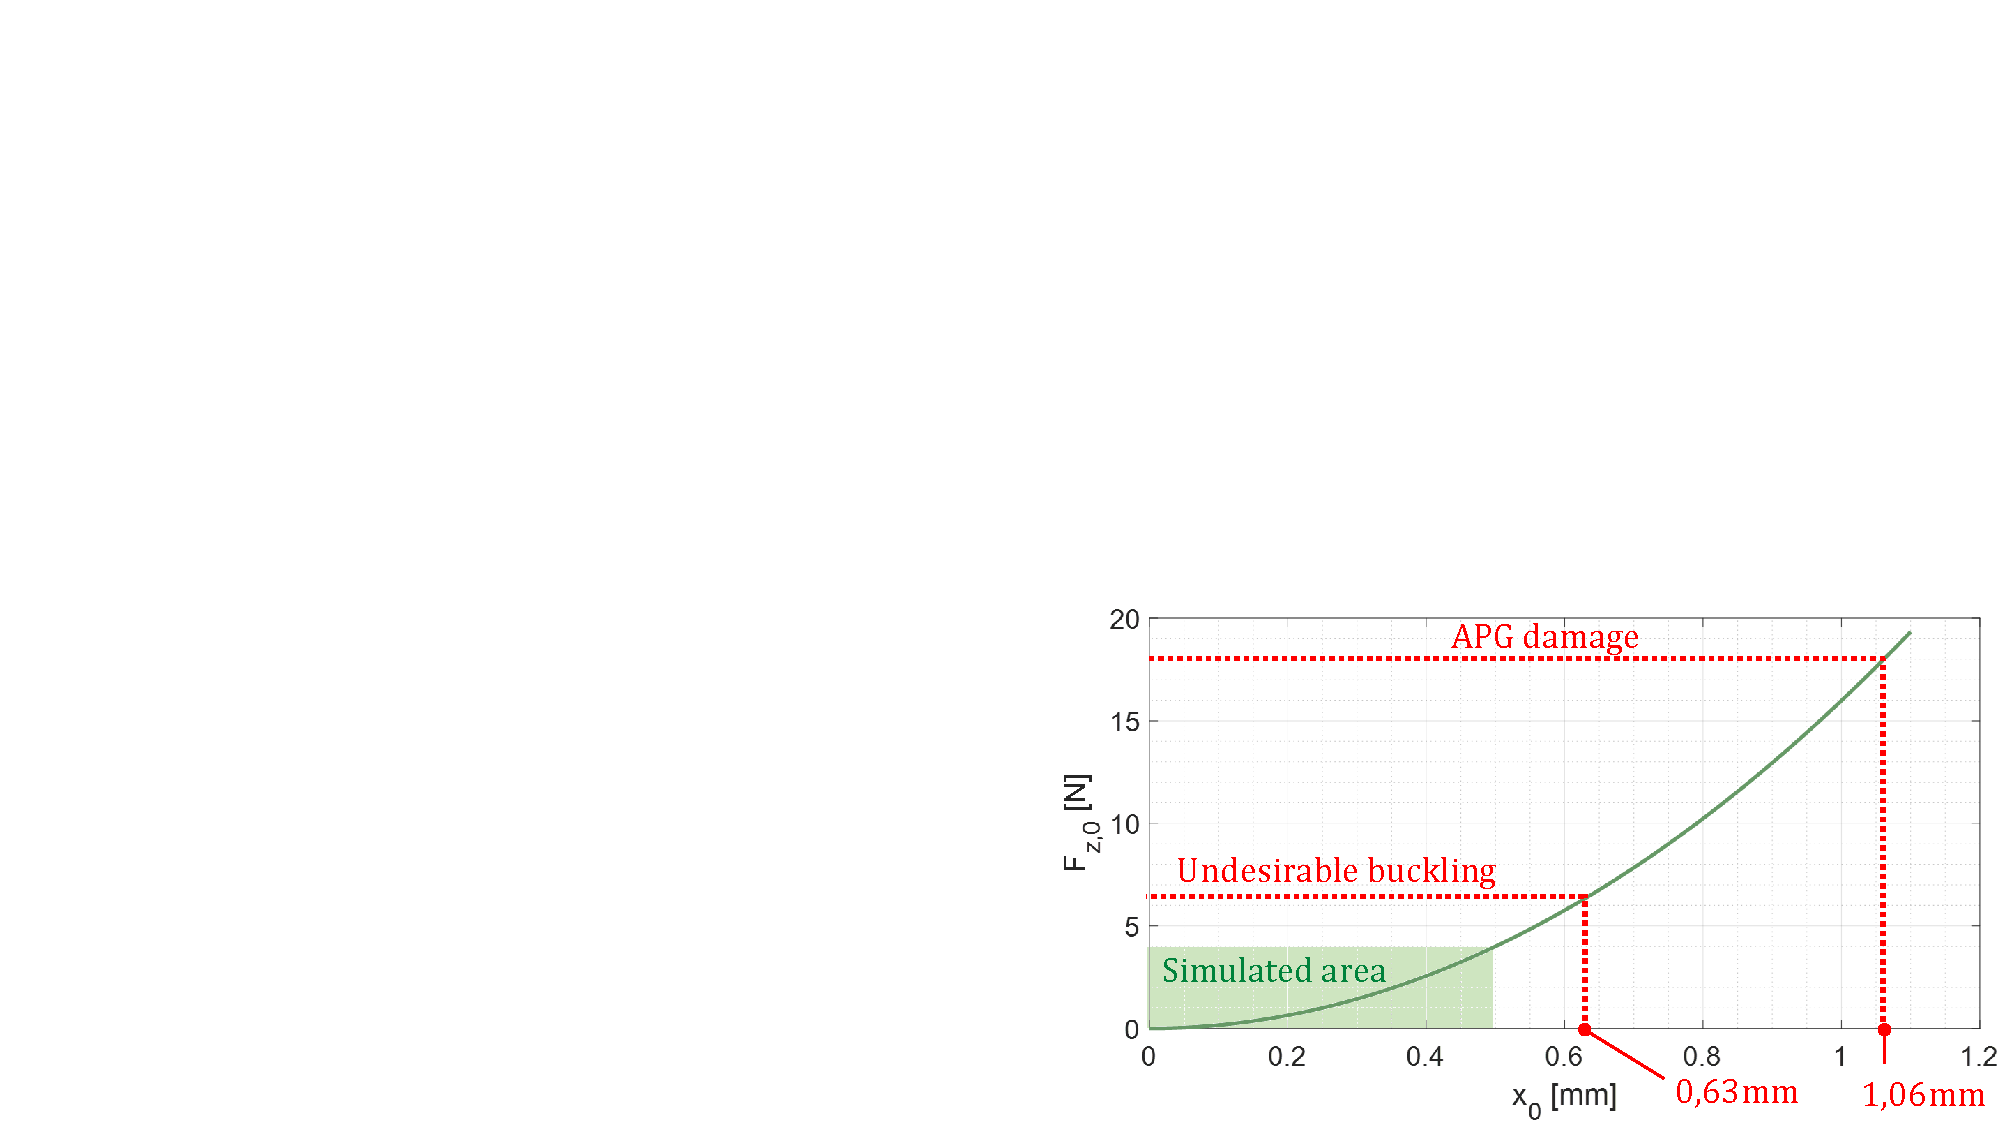
\includegraphics[trim={17.9cm 0cm 0cm 10cm},clip,width=0.9\linewidth]{figures/buckling_limit.pdf}
	\caption{APG elastic counter reaction on $\vec{z}$ axis at $x_m=0$, depending on the initial structural buckling height $x_0$}
	\label{fig:buckling_limit}
\end{figure}
%%%%%%%%%%%%%%%%%%%%%%%%%%%%%%%%%%%%%%
% Ltex language=en

    %///////////////////////////////////////////// 
	\subsection{Experimental characterizations}	
	\label{subsec:Experimental characterizations}
    %/////////////////////////////////////////////
The experimental test bench for the electromechanical characterizations of the electromechanical converter is presented on figure \ref{fig:BDT_OB+GPA}. An additional beam is mounted with the APG in order to prevent its rotation around any axis. A micrometric screw helps to set the initial structural buckling level $x_0$ ($\pm 10$µm). The bearing decouples the rotation of the screw with the rotation of the beam structure in order to prevent unwanted torsional stress. Two symmetrically mounted masses are added on the initial central mass with a 45\degree{} machined plane. The latter receives and reflects the displacement sensor emitted laser along the $\vec{z}$ axis and allows to get the $x_m$ position of the mas along $\vec{x}$ axis ($\pm 10$µm). The APG power is dissipated in the $R_l$ resistor and the $U_p$ tension ($\pm 1$mV), along with $x_m$, are monitored through a data acquisition card NI-USB 6212 and a LabVIEW interface. Finally, the two HC plungers actuate the mass from one stable equilibrium position to the other.
%%%%%%%%%%%%%%%%%%%%%%%%%%%%%%%%%%%%%%
\begin{figure}[!htbp]
	\centering
	\captionsetup{justification=centering}
	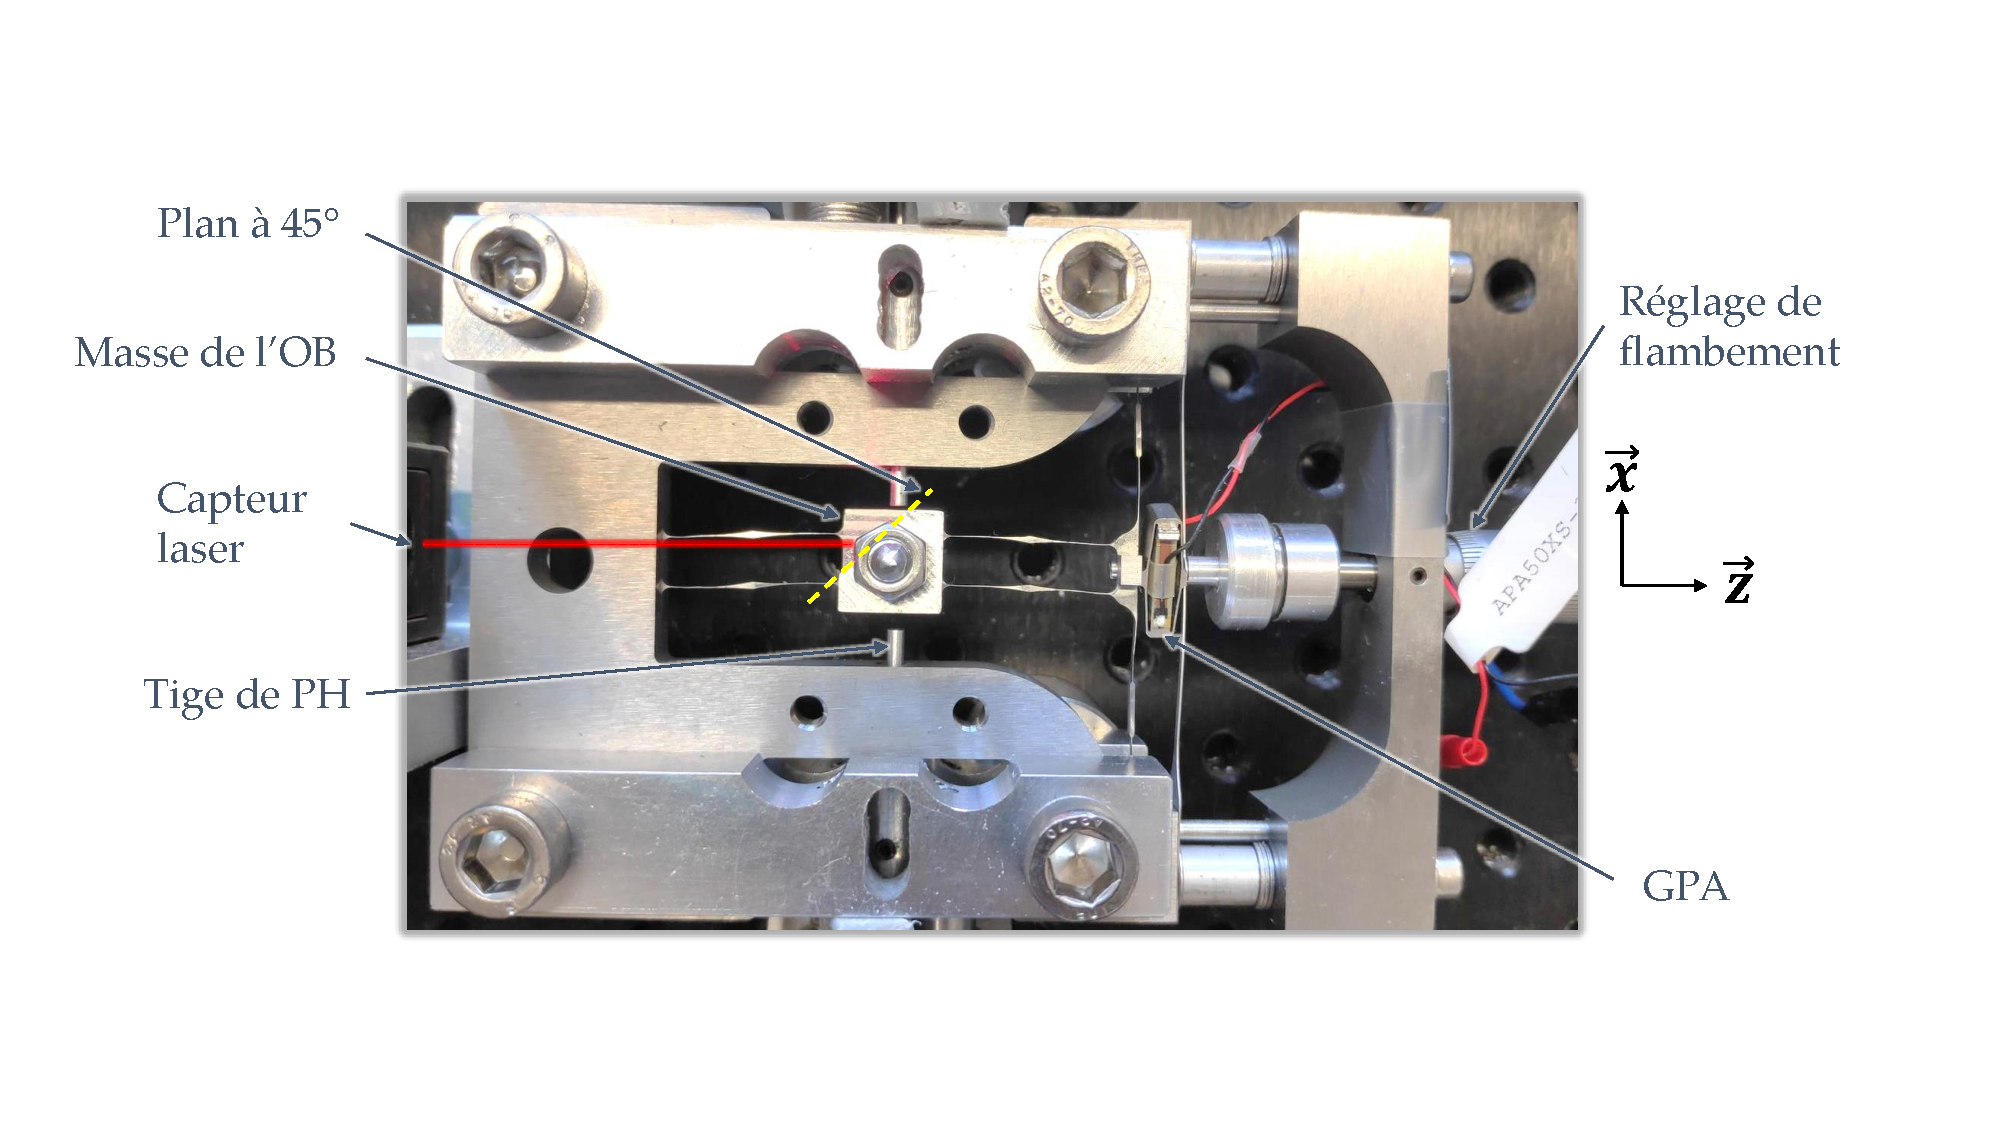
\includegraphics[trim={2cm 0cm 0cm 5.5cm},clip,width=\linewidth]{figures/BDT_OB+GPA.pdf}
	\caption{Test bench of the electromechanical converter}
	\label{fig:BDT_OB+GPA}
\end{figure}
%%%%%%%%%%%%%%%%%%%%%%%%%%%%%%%%%%%%%%%
The HV mechanical influence is not considered in order to isolate the electromechanical converter dynamic behavior. The mass is guided by a HC from a stable equilibrium position until it reaches \mbox{$x_m=0$}, and then oscillates around the opposite stable equilibrium position. The experimental data was used to identify and recalibrate the following electromechanical parameters of the harvester, through iterative simulations of the global \mbox{model :} $Q$, $f_0$, $K$ and $k_{sys}^2$ (tab. \ref{tab:parametres_lacher_free}). The experimental oscillation frequency $f_0$ and energy conversion efficiency $\eta_{br}$ can also be calculated.
%%%%%%%%%%%%%%%%%
\begin{table}[!htbp]
\centering
\captionsetup{justification=centering}
\resizebox{.8\linewidth}{!}{%
	\begin{tabular}{ c | c | c }
	\toprule
	& \textbf{Simulation with}  	   & \textbf{Simulation with}       \\
	& \textbf{theoretical}  		   & \textbf{recalibrated }		 	\\
	\multirow{-3}{*}{\textbf{Symbol}}
	& \textbf{parameters}			   & \textbf{parameters} 			\\
	\midrule
	$Q$                       & 50.0                  & 30.0 		  	\\  
	$f_0$                     & 47.0 Hz               & 27.9 Hz  		\\
	$x_0$                     & 0.49 mm               & 0.50 mm    		\\
	$K$                       & 2.56e5 N/m            & 0.85e5 N/m 		\\
	${k^2_{sys}}$             & 16 \%                 & 1.25 \% 		\\
	$\eta_{br}$               & 75 \%                 & 12.9 \%   		\\
	\bottomrule
	\end{tabular}}
	\caption{Theoretical and experimentally recalibrated values of the electromechanical converter.}
	\label{tab:parametres_lacher_free}
\end{table} 
%%%%%%%%%%%%%%%%%%%%%  
    %///////////////////////////////////////////// 

	\subsection{Analyze and summary}	
	\label{subsec:Analyze and summary}
    %/////////////////////////////////////////////
The experimental dynamic behavior of the converter is predictable by the equations established after identification of the system parameters listed in table \ref{tab:parametres_lacher_free}. However, the performances of the experimental prototype are below the theoretical expectations (tab. \ref{tab:parametres électromécaniques}). The efficiency drop is consistent with the quality factor and the electromechanical coupling coefficient drop (eq. \ref{eq:eta_ob}). 

Two major factors could have led to such results. First, the quality factor decrease could be related to the general non-permanent assembly that uses non-perfect embeddings with fixation screws and a mobile micrometric screw. Then, small undulations have been observed on the BBs after fabrication and could also have gotten worse during the manipulation. These undulations reduce $K_{bb}$, diminishing $k^2_{sys}$ according equations \ref{eq:k2_sys}-\ref{eq:K_eq}. Improvements are proposed later in order to reduce the energy losses during this stage.

%/!\/!\/!\/!\/!\/!\/!\/!\/!\/!\/!\/!\/!\/!\/!\/!\/!\/!\/!\/!\/!\/!\/!\/!\%
\section{EXPERIMENTAL APPROACH FOR THE HV \mbox{DESIGN}}
\label{sec:EXPERIMENTAL APPROACH FOR THE HV DESIGN}
%/!\/!\/!\/!\/!\/!\/!\/!\/!\/!\/!\/!\/!\/!\/!\/!\/!\/!\/!\/!\/!\/!\/!\/!\%
In order to validate the feasibility of the HVs we adopted an experimental approach to find the material and geometrical parameters of the tube capable to achieve $(r_{Cf})_{min}=26$ (tab. \ref{tab:parametres_hydrauliques}). A HV composed of a kapton tube \cite{Dupont2012} of initial diameter $D_t=1.05$mm and thickness $th_t=25$ µm was found to meet this hydraulic criteria. It will be called HV$_{T1}$ afterwards. 
    %///////////////////////////////////////////// 
	\subsection{HV hydraulic experimental characterization}	
	\label{subsec:HV hydraulic test bench presentation}
    %/////////////////////////////////////////////
Figure \ref{fig:essais_hydraulique_VH} shows the HV$_{T1}$ during the experimental characterizations on the hydraulic test bench. An electromechanical rotary plate is monitored on LabVIEW interface and imposes the bending angle $\theta$. A liquid filled syringe is emptied through the HV$_{T1}$ and its exciting flow rate $q_{ser}$ is deduced by tracking its moving piston displacement. The pressure loss coefficient $Cf_{T1}$ is calculated as \mbox{follows :}
\begin{equation}
	Cf_{T1} = \dfrac{p_1-p_2}{q_{ser}^2}
\end{equation}
Where $p_1$ and $p_2$ are respectively the fluid pressure monitored before entering and after exciting the HV$_{T1}$.
%%%%%%%%%%%%%%%%%%%%%%%%%%%%%%%%%%%%	
\begin{figure*}[!htb]
\begin{center}
	\captionsetup{justification=centering} 
	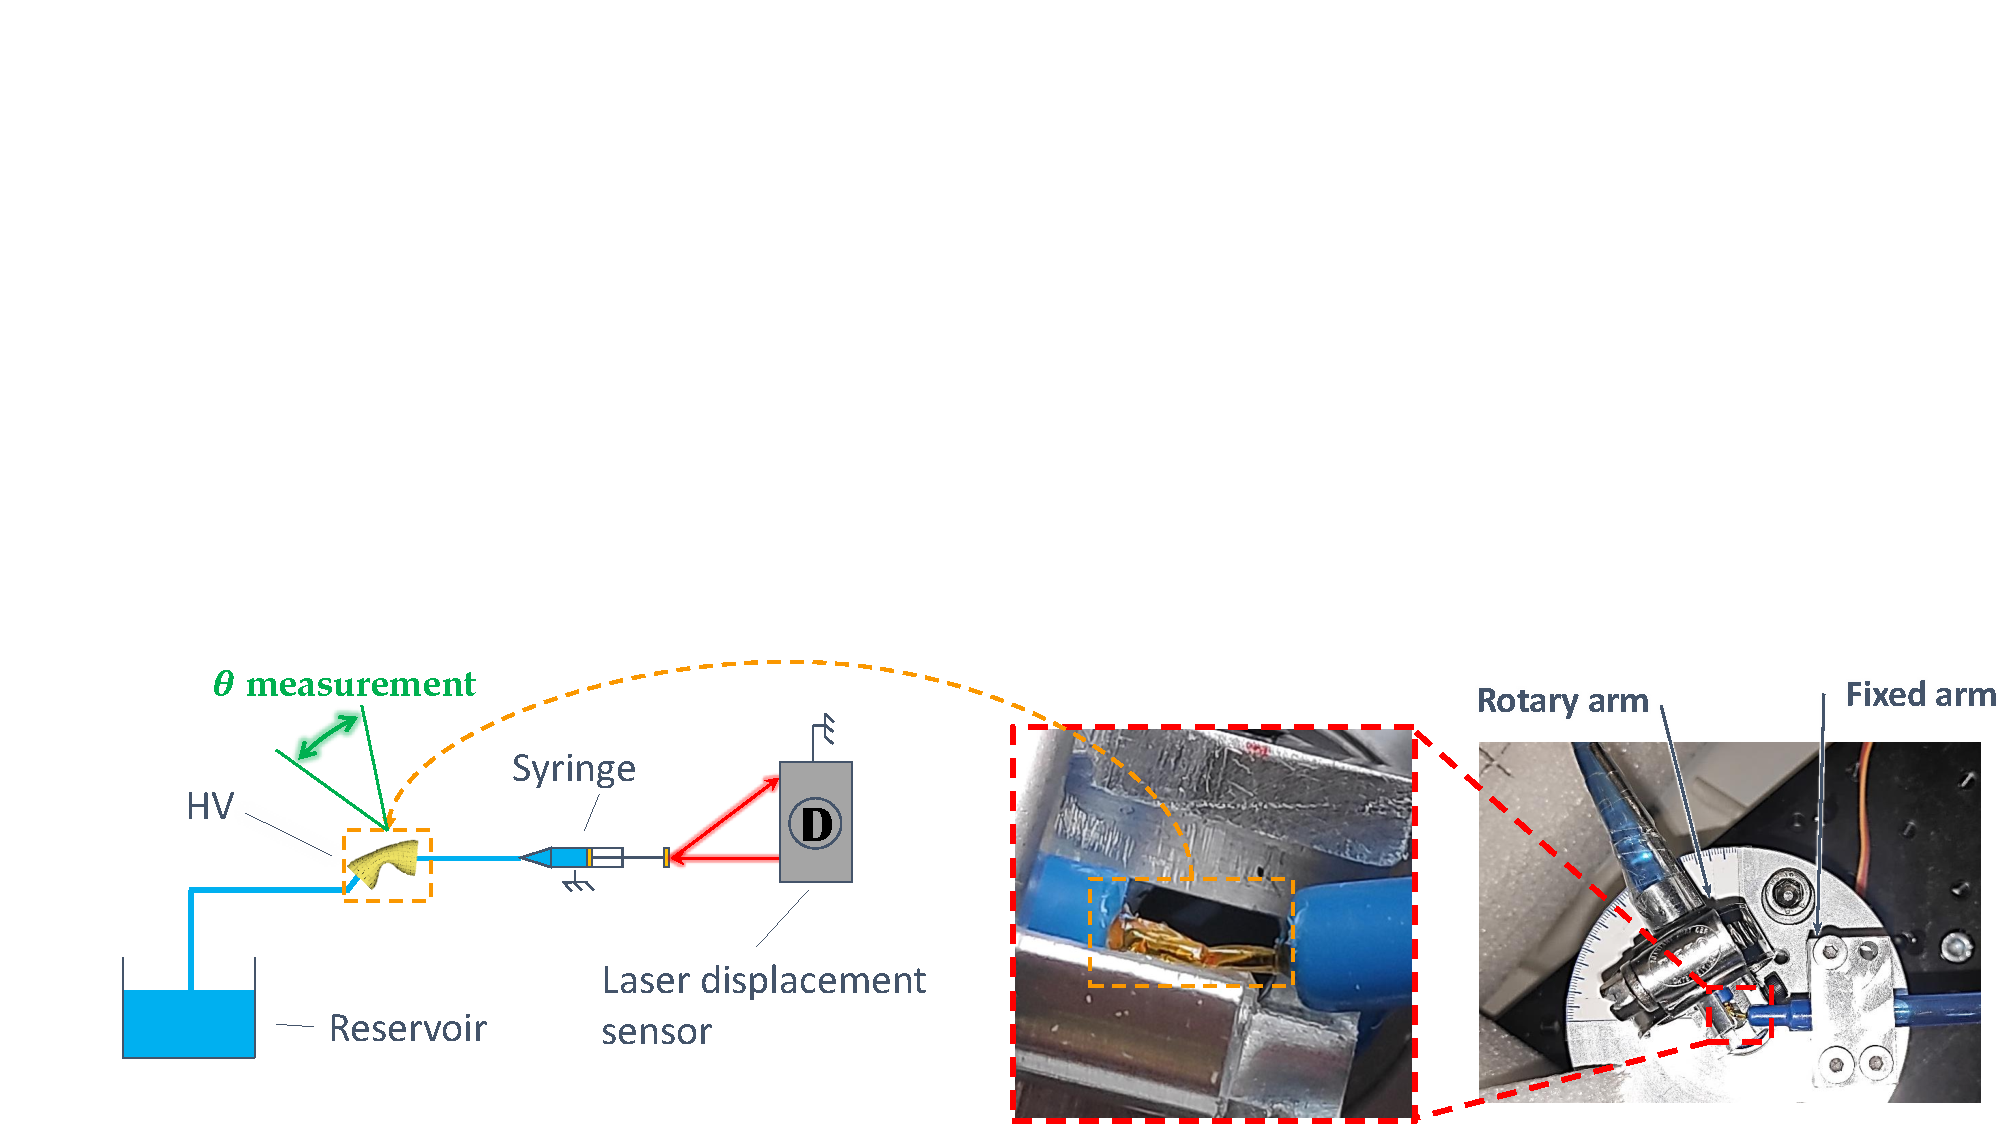
\includegraphics[trim={2cm 0cm 0cm 11cm},clip,width=.8\textwidth]{figures/essais_hydraulique_VH.pdf}
	\caption{Hydraulic characterization test bench for HVs}
	\label{fig:essais_hydraulique_VH}
\end{center}	
\end{figure*}    
%%%%%%%%%%%%%%%%%%%%%%%%%%%%%%%%%%%% 
The emptying procedure was repeated 7 times for $\theta$ varying from $0^{\circ}$ to $60^{\circ}$ with $10^{\circ}$ increments. The experimental results are plotted on figure \ref{fig:resultats_essais_hydraulique_VH_D1mm}.
%%%%%%%%%%%%%%%%%%%%%%%%%
\begin{figure}[!htbp]
\centering
	\captionsetup{justification=centering}
	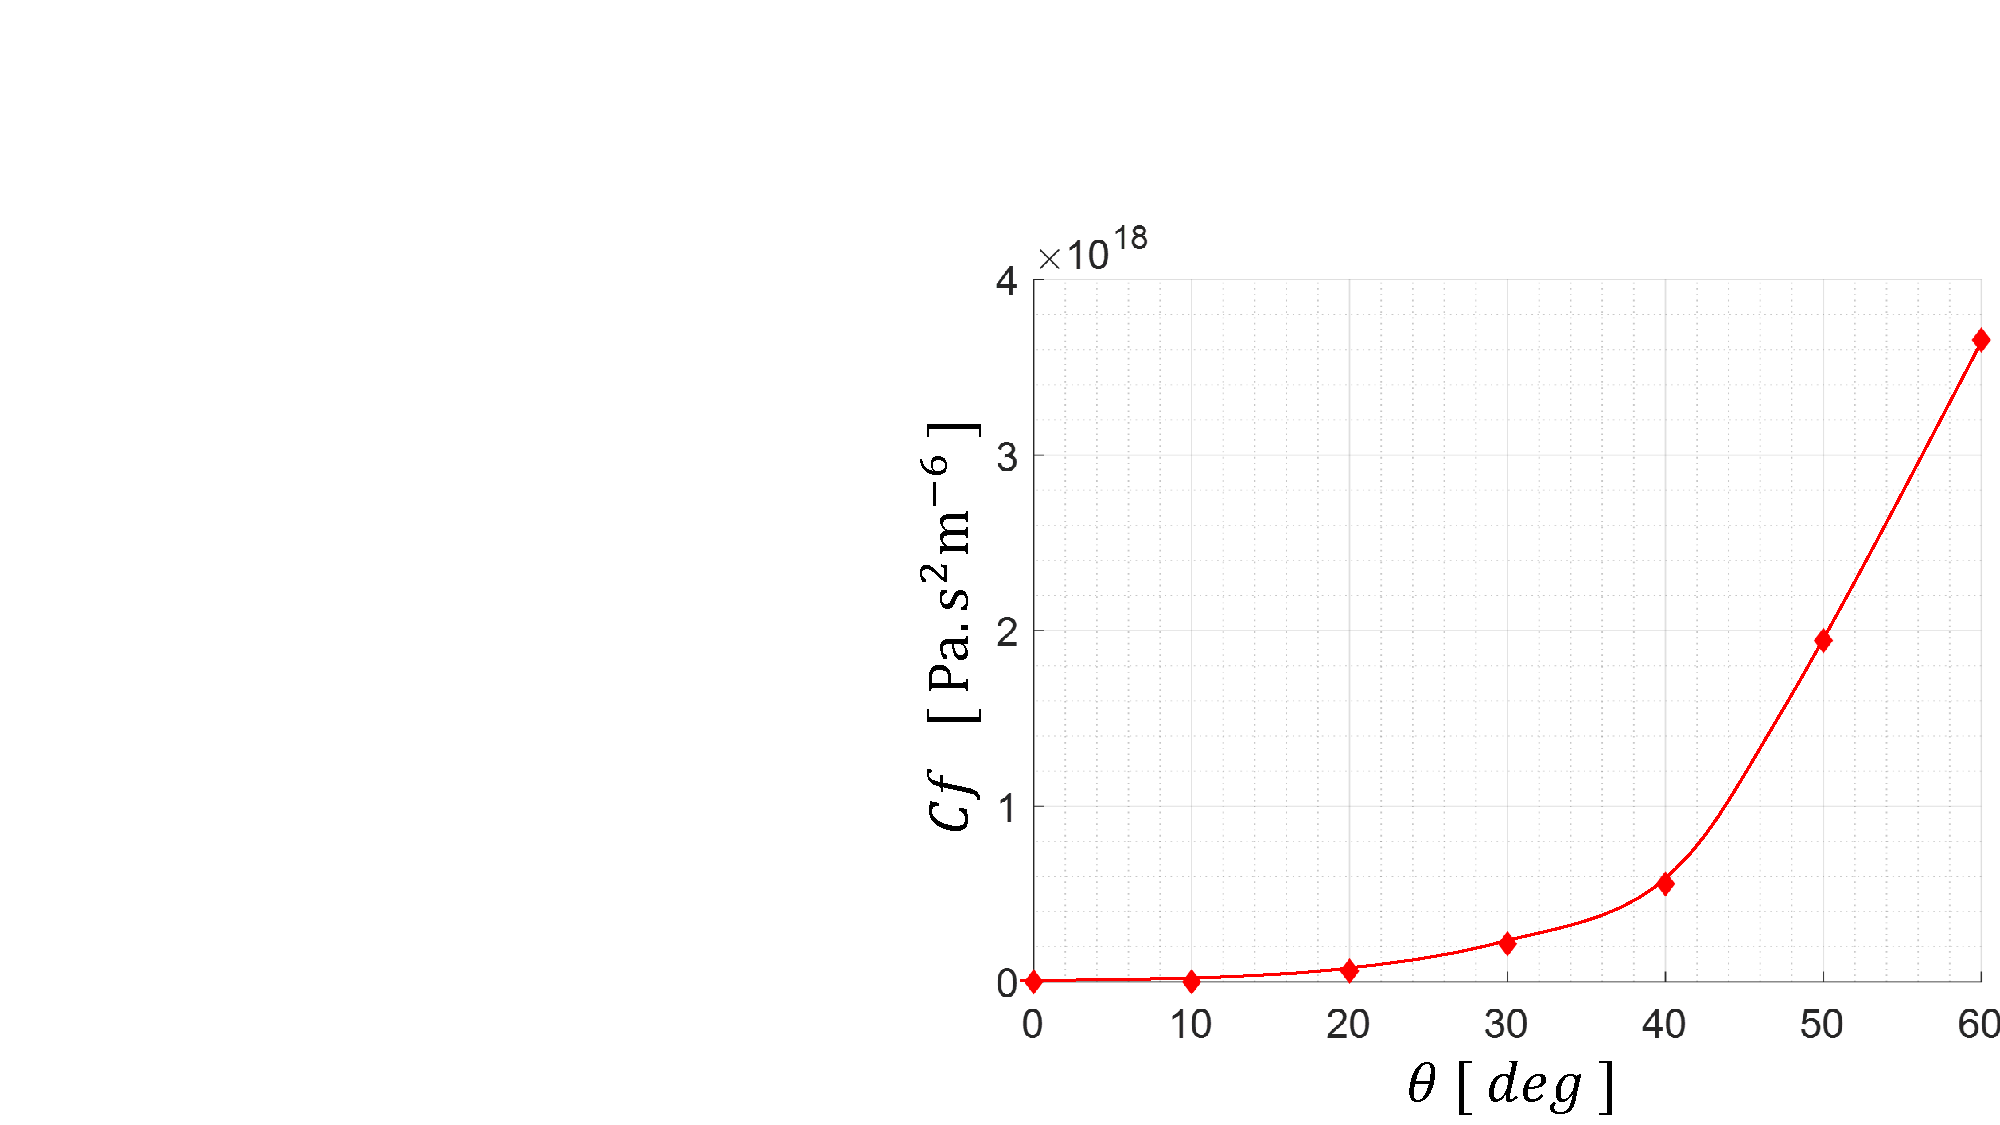
\includegraphics[trim={15.5cm 0cm 0cm 3.6cm},clip,width=0.6\linewidth]{figures/resultats_essais_hydraulique_VH_D1mm.pdf}
	\caption{Hydraulic characterization of the HV$_{T1}$.}
	\label{fig:resultats_essais_hydraulique_VH_D1mm}
\end{figure}
%%%%%%%%%%%%%%%%
The hydraulic restriction coefficient of the HV$_{T1}$ has been evaluated to 60 if the opened angle $\theta_0=20^{\circ}$ and the closed angle $\theta_c = 60^{\circ}$. Its hydraulic behavior respects the minimum criteria of \mbox{$(r_{Cf})_{min}=26$} and therefore can ensure the adequate hydraulic commutation to cycle the BR mass motion. In order to set an optimal angle operation range $\Delta\theta$ we must investigate the evolution $K_{HV}(\theta)$. This matter will not be discussed in this paper. However, $\Delta\theta$ must be minimized in order to limit the energy needed for the HVs operation and also, $\theta_0$ must be minimized to reduce the hydraulic energy losses in the active branch.

The following section presents the recalibrated harvester model using the hydraulic characterization data of the HV$_{T1}$ and the electromechanical experimental data of the BR with the APG.

%/!\/!\/!\/!\/!\/!\/!\/!\/!\/!\/!\/!\/!\/!\/!\/!\/!\/!\/!\/!\/!\/!\/!\/!\%
\section{MODEL RECALIBRATION WITH EXPERIMENTAL DATA}
\label{sec:MODEL RECALIBRATION WITH EXPERIMENTAL DATA}
%/!\/!\/!\/!\/!\/!\/!\/!\/!\/!\/!\/!\/!\/!\/!\/!\/!\/!\/!\/!\/!\/!\/!\/!\%

The experimentally identified parameters have been implemented in the global multiphysic coupled model to enhance its predictability and to evaluate the harvester performances. The last matter is achieved by evaluating the mechanical influence of the HV$_{T1}$ through an experimental approach in order to identify the energy losses at the HV-mass contact point (T on figure \ref{fig:HV_actuation_detail}). 

	%/////////////////////////////////////////////
	\subsection{Experimental evaluation of the mechanical impact of HV$_{T1}$}
	%/////////////////////////////////////////////
The HV$_{T1}$ has been mounted on the experimental test bench presented on figure \ref{fig:BDT_OB+GPA} and two experimental trials have been performed to identify the HV mechanical influence : free oscillations and oscillations with HV$_{T1}$ presence, during a harvesting phase. The mass is initially set on $x_m=x_0$ and then pushed toward $x_0$. The HV$_{T1}$ internal pressure is adjusted to 30kPa with an oil column, in order to be consistent with the simulated case (tab. \ref{tab:parametres_hydrauliques}). The oscillation phase begins when the mass crosses the $x_m=0$ position. In order to set $\theta_0$ we add an angle stopper that is shown in figure \ref{fig:contact_M_VH_lachers}. $\theta_c$ is then reached when the oscillations stop at $x_m=x_0$. The mass position and the APG tension are monitored during the tests.
%%%%%%%%%%%%%%%%%%%%%%%%%%%%%%%%%%%%	
\begin{figure}[!htbp]
	\begin{center}
		\captionsetup{justification=centering}
		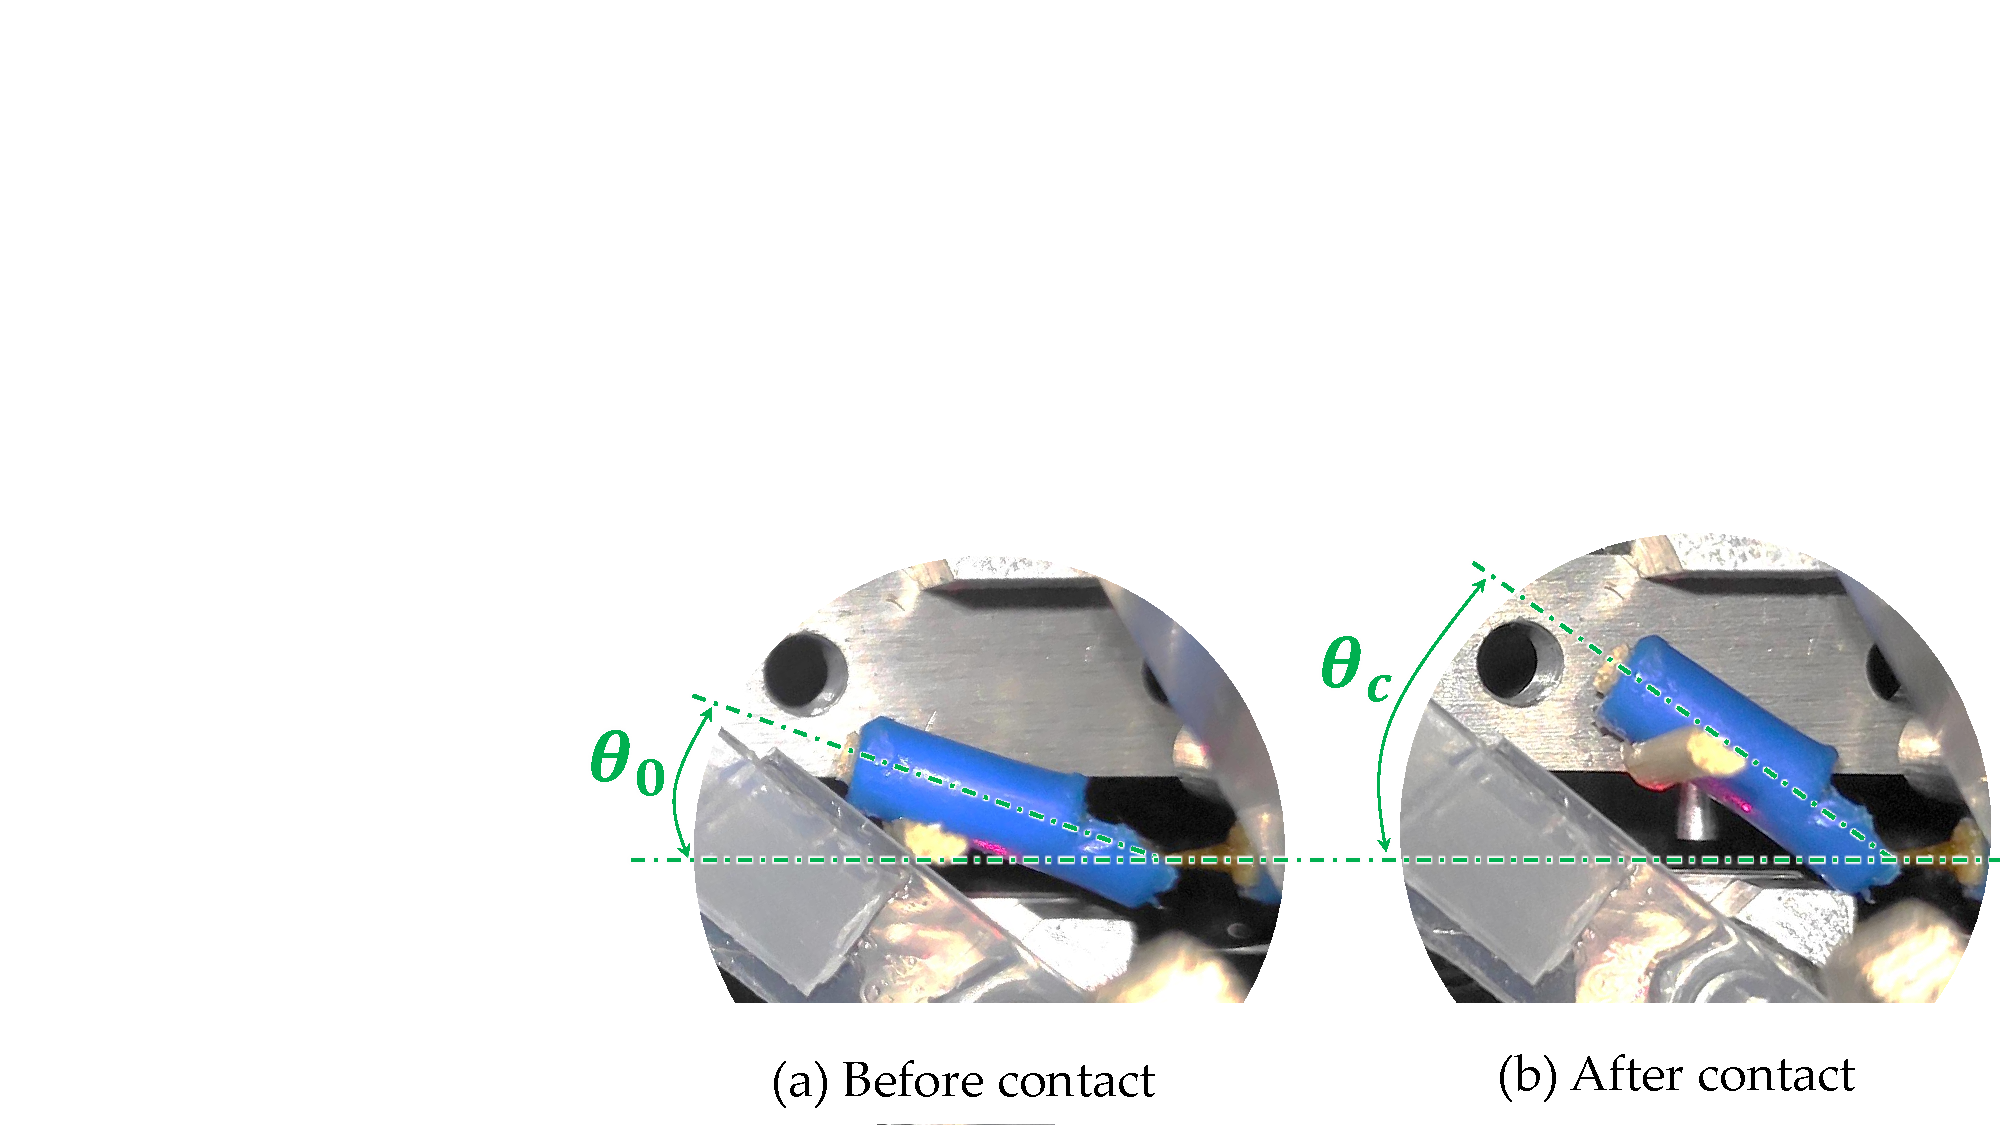
\includegraphics[trim={6.9cm 0cm 0cm 9cm},clip,width=0.9\linewidth]{figures/contact_M_VH_lachers.pdf}
		\caption{HV$_{T1}$ picture for (a).$\theta_0(x_m=-x_{0})$ and for (b).$\theta_f(x_m=x_0$).}
		\label{fig:contact_M_VH_lachers}
	\end{center}
\end{figure}
%%%%%%%%%%%%%%%%%%%%%%%%%%%%%%%%%%%%

The global model parameters listed in table \ref{tab:parametres lacher tube} are recalibrated for both test configurations by iterative simulations. 
The simulations with the recalibrated parameters and the experimental data are superposed on figure \ref{fig:BDT_OB+GPA} concerning the harvesting phase of both configurations. 

After recalibration, the low error between the simulated and the experimental data verify that the electromechanical dynamics behavior of the harvester is theoretically predictable by the established model. 
The comparison between the results of the two tests reveal the mechanical impact of the HV. 
The stiffness at $\theta_c$ is calculated with $x_0$ evolution between the two tests and equation \ref{eq:OB-GPA}. 
The quality factor decrease is a result of the rubbing between the mass and the HV and diminishes the BR energy conversion efficiency.
The HV adds a supplementary dynamic mass in the BR.
The electromechanical coupling coefficient is not influenced by the HV presence, which is consistent with equation \ref{eq:k2_sys}.  
%%%%%%%%%%%%%%%%%%%%%%%%%%%%%%%%%%%%%%
\begin{figure}[!htbp]	
\captionsetup{justification=centering}
	\begin{subfigure}{.49\linewidth}
		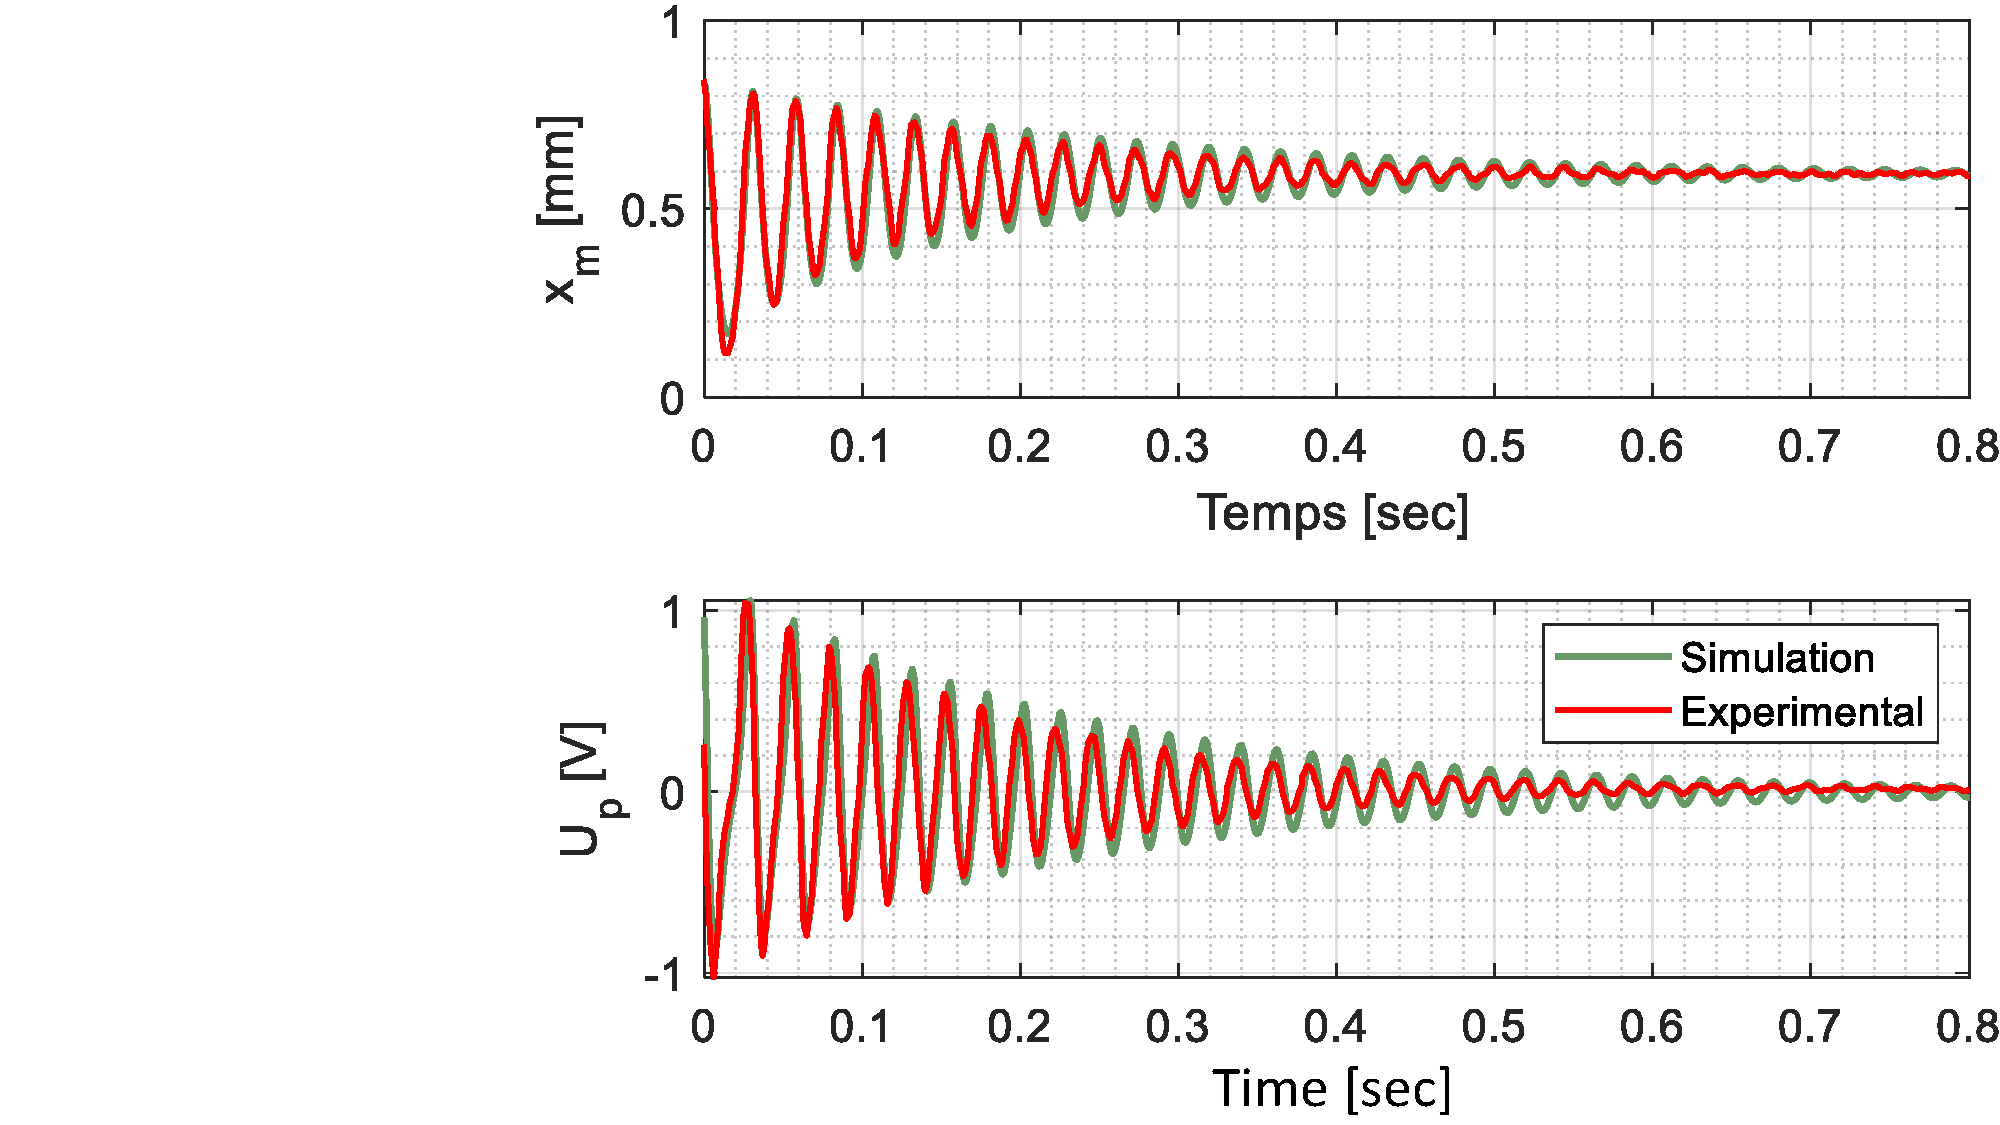
\includegraphics[trim={9cm 0cm 0cm 0cm},clip,width=\linewidth]{figures/recalage_free.pdf}
		\caption{Free oscillations}
		\label{fig:recalage_free}
	\end{subfigure}
	\begin{subfigure}{.49\linewidth}
		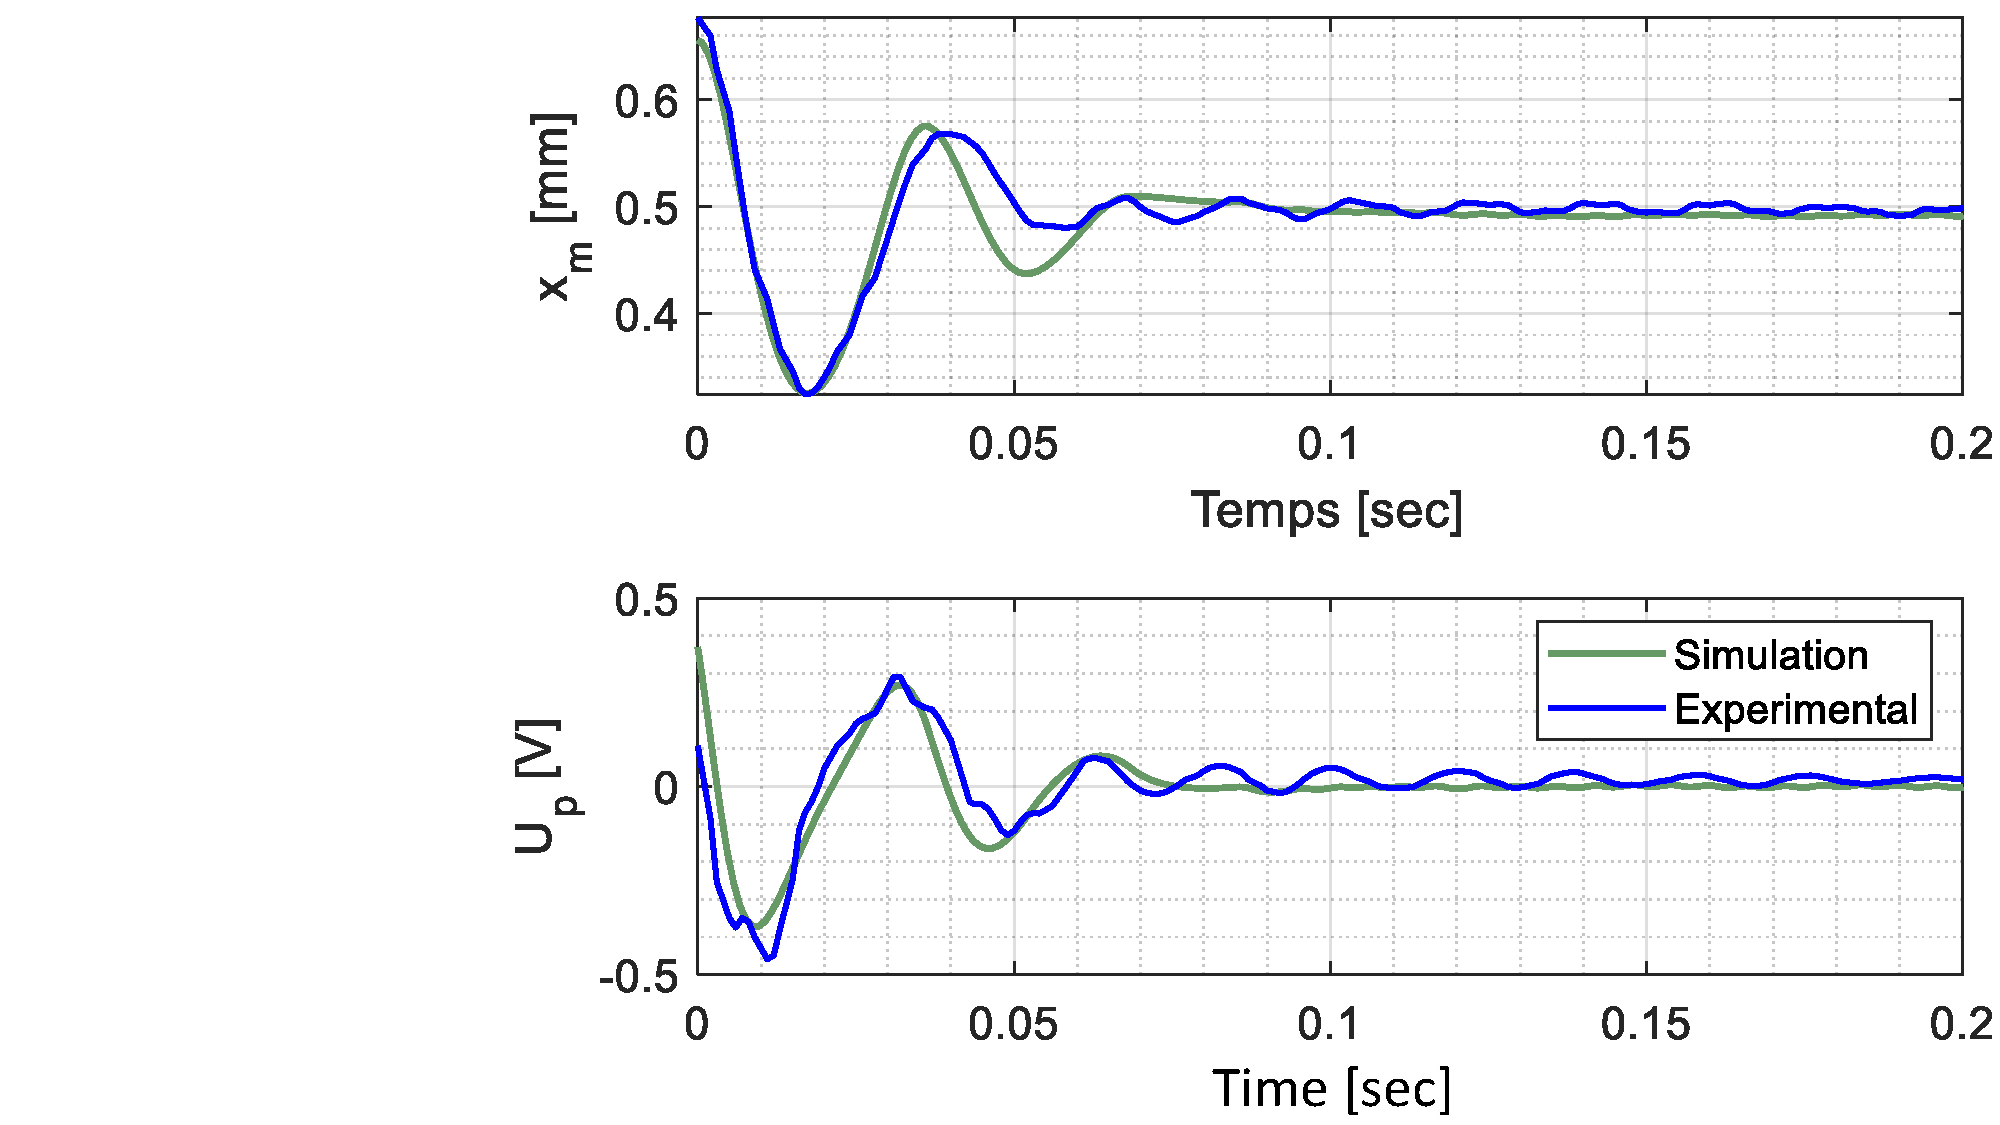
\includegraphics[trim={8.6cm 0cm 0cm 0cm},clip,width=\linewidth]{figures/recalage_tube.pdf}
		\caption{Oscillations with HV$_{T1}$ presence}
		\label{fig:recalage_tube}
	\end{subfigure}
	\caption{Experimental measurements and global system simulation with the identified parameters of table \ref{tab:parametres lacher tube}.}
	\label{fig:recalage_global}
\end{figure}
%%%%%%%%%%%%%%%%%%%%%%%%%%%%%%%%%%%%%%%

	%/////////////////////////////////////////////
	\subsection{Recalibrated coupled model}
	%/////////////////////////////////////////////
%%%%%%%%%%%%%%%%%%%%%%%%%%%%%%%%%%%
\begin{table}[!htbp]
	\centering
	% \resizebox{\textwidth}{!}{%
		\begin{tabular}[t]{c|c|c}
\toprule
\multicolumn{1}{c}{\textbf{Parameter}}	&
\multicolumn{1}{c}{\textbf{BR}} 	& 
\multicolumn{1}{c}{\textbf{BR+VH$_{T1}$}}  \\
\midrule
$D_r$ [mm] 						& \cellcolor{ashgrey} 		& {4} 		\\ \hline
$\Delta\theta$ [deg] 			& \cellcolor{ashgrey} 		& {{[$\approx$ 19 ; $\approx$ 36]}} \\ \hline
$K_{T1}(\theta_c)$ [Nmm/rad]	& \cellcolor{ashgrey}  		&  0.27 		\\ \hline
$a$ [mm]         			    & \cellcolor{ashgrey}  		&  2.24		\\ \hline
$f_d$ [-] 						& \cellcolor{ashgrey}  		&  0.42  		\\ \hline
$K$ [N/m] 						&	84480			  	 	&  84480  			\\ \hline
$x_0$ [mm] 						& {0.59}					& {0.50}  	\\ \hline
$Q$	[-] 						& 		24.0		 		& 5.0     					\\ \hline
$k^2_{sys}$ [\%] 				& 		1.25		 		& {1.25}   	\\ \hline
$\eta_{br}$ [\%] 				& 		11.9		 		& 2.6   \\ \hline	
$R_l$ [k$\text{\ohm}$] 			&	{15.5}					& {15.5}   	\\ \hline		
$m$	[g]						    &	{5.88}					& 9.00   		\\ \hline	
$f_0$ [Hz]						&		32.9				& 27.9   					\\
\bottomrule	
	\end{tabular}
        \caption{Value des paramètres de l'OB et de l'ensemble OBVH implémentant le tube T100p suite au essais de lâchers expérimentaux}
        \label{tab:parametres lacher tube}
\end{table}        
%%%%%%%%%%%%%%%%%%%%%%%%%%%%%%%%%%%%	
%/!\/!\/!\/!\/!\/!\/!\/!\/!\/!\/!\/!\/!\/!\/!\/!\/!\/!\/!\/!\/!\/!\/!\/!\%
\section{CONCLUSION}
\label{sec:CONCLUSION}
%/!\/!\/!\/!\/!\/!\/!\/!\/!\/!\/!\/!\/!\/!\/!\/!\/!\/!\/!\/!\/!\/!\/!\/!\%


%% If you have bibdatabase file and want bibtex to generate the
%% bibitems, please use
%%
%%  \bibliographystyle{elsarticle-num} 
%%  \bibliography{<your bibdatabase>}

%% else use the following coding to input the bibitems directly in the
%% TeX file.

%\begin{thebibliography}{00}
\bibliography{biblioArticle1.bib}
\bibliographystyle{elsarticle-num}
%\bibliographystyle{unsrt} 
%\end{thebibliography}


\end{document}
\endinput